\chapter{The Split Ring Resonator}


In the work done by Xu et al \cite{Xu2021}, the plasma discharge was generated using a CCP jet, specifically a design by the European Cooperation in Science and Technology (COST) \cite{Gorbanev2019}. The COST plasma jet was originally developed for medical and biomedical applications, as such were developed to operate at the approved ISM frequency of 13.56 MHz. However, RF plasma sources are flawed in the sense that they have a limited plasma density, which could theoretically limit the rate of splitting of CO$_2$ molecules.

To improve upon this, the plasma discharge used for this project would use a micowave plasma, specifically a microstrip-based source called the \textit{split ring resonator} (SRR). Using such a device will have two main benefits. First, the power efficiency of the microwave plasmas would allow for discharges would either allow for lower operating powers or greater electron densities at the same operating power. Additionally, the device would also be much smaller and cheaper to manufacture.

An illustration of an SSR can be seen in figure \ref{fig:SRR}. The design of a SRR is quite simple, consisting of a conducting ring, usually made of copper, laid on top of a dielectric substrate. The bottom of the dielectric consist of a ground plane that covers the entirety of the surface. This has the added benefit of dispersing the heat generated from the SRR. As seen in figure \ref{fig:SRR}, there is a small gap made on the top surface that breaks the copper ring, which is where the plasma discharge occurs. 


\begin{figure}[h!]
	\centering
	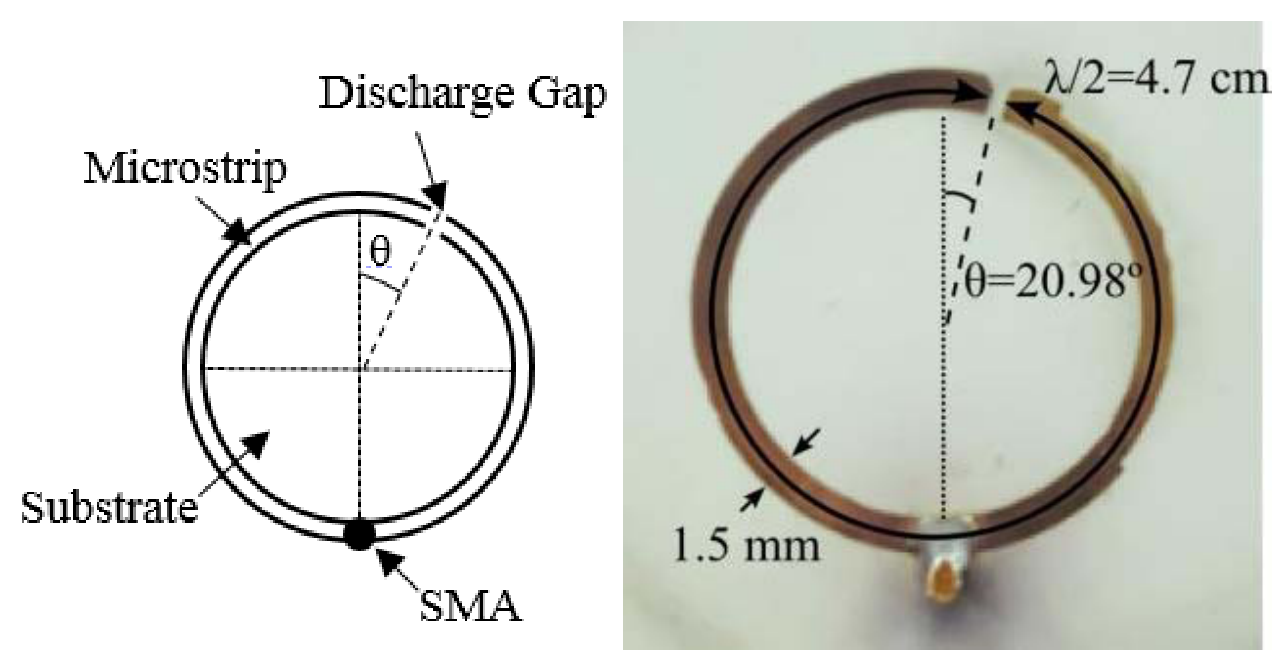
\includegraphics[width=0.7\linewidth]{chapter_4/figures/split_ring_resonator.png}
	\caption{Schematic (left) and photo (right) of SRR \cite{Dextre2017}.}
	\label{fig:SRR}
\end{figure}

\section{Overview}


In order to achieve a discharge, a high frequency (microwave) voltage is applied to the SRR via the SMA connector. The exact frequency to be used is governed by two factors: the mean circumference of the top conducting ring and the dielectric constant of the substrate used. The mean circumference is specifically designed to be half the wavelength corresponding to the desired frequency. The dielectric constant is required to determine the speed of light in the dielectric medium used. Thus, an equation for the frequency used for a given SRR is \cite{Dextre2017}:

\begin{equation}
     f = \frac{c}{\lambda\sqrt{\varepsilon_r}}
     \label{eq:resonant_frequency}
\end{equation}

The reason why the mean circumference is designed to be half the desired wavelength is for power efficiency. Due to this design, the ends of the SRR (i.e. where the gap is) will be $180^\circ$ out of phase from each other. Because of this, when one end of the SRR is at the peak of the AC cycle, the other will be at a trough; thus the potential difference between the two ends has been doubled. This geometric design allows for the doubling of the strength of the electric field at a constant power. 

Astute readers may notice that the ring of the SRR device shown in figure \ref{fig:SRR} is not symmetrical. Instead, the discharge gap appears to be offset towards one side of the device. This is deliberate as the offset position changes the characteristic impedance of the device, allowing for impedance matching without the need of additional passive components. This offset angle ($\theta$),  measured from the very centre of the ring, is chosen using the expression \cite{Iza2005}:

\begin{equation}
	\theta = arccos(1 - \frac{Z_{in} \pi}{Z_0 Q})
	\label{eq:offset_angle}
\end{equation}

where $Z_{in}$ is the input impedance of the power supply, $Q$ is the quality factor, and $Z_0$ is the characteristic impedance of the SRR. 

The input impedance of most power supplies is 50 $\Omega$, while the quality factor is a parameter given on the data sheet of the substrate used. As for the characteristic impedance, it is governed by four factors:

\begin{itemize}
    \item the width of the top copper trace, $w$.
    \item the thickness of the copper pour, $t$.
    \item  the thickness (or height) of the dielectric substrate, $h$.
    \item the dielectric constant of the substrate, $\varepsilon_r$.
\end{itemize}

For a thin microstrip, it is typical to use the analytical solution derived by Wheeler \cite{wheeler_1977}, as it approximates the characteristic impedance with an error of less than 1\%. These are shown in equations \ref{eq:wheeler_microstrip}-\ref{eq:wheeler_effective_w}: 

\begin{equation}
    Z_0 = \frac{42.4}{\sqrt{1+\varepsilon_r}}ln\left( 1 + \frac{4h}{w'}(X_1 + X_2)\right)
    \label{eq:wheeler_microstrip}
\end{equation}
\begin{equation}
    X_1 = \frac{4h}{w'}\left(\frac{14\varepsilon_r + 8}{11\varepsilon_r}\right)
\end{equation}
\begin{equation}
    X_2 = \sqrt{\left(\frac{4h}{w'}\right)^2 \left(\frac{14\varepsilon_r + 8}{11\varepsilon_r}\right)^2 + \pi^2\frac{1+\frac{1}{\varepsilon_r}}{2}}\
\end{equation}
\begin{equation}
    w' = w + \frac{t}{\pi}ln\left(\frac{4e}{\sqrt{(\frac{t}{h})^2 + (\frac{t}{w\pi + 1.1\pi})^2}}\right)\frac{\varepsilon_r + 1}{2\varepsilon_r}
    \label{eq:wheeler_effective_w}
\end{equation}


\section{Production}

While the SRR device shown in figure \ref{fig:SRR} would generate a microwave plasma, a slight modification is required for the device to be usable as a small jet for this project. To allow the gases to flow through the plasma and exit the device, an orifice needs to be placed in the discharge gap.

While this may be a small alteration to the device, it was an unknown if such a change would effect the behaviour of the plasma formed. To investigate this, several simulations were run to better understand the discharge dynamics. For this research, the author used \textit{Particle-in-cell} (PIC) simulations using the software called \textit{XOOPIC} \cite{Verboncoeur1995}. Further information on PIC simulations and XOOPIC can be found in the appendices.



%The SRR device used in this project introduces a slight modification to the design of the traditional SRR. In order to create a small jet of plasma, an orifice needs to be placed in the region of the gap of the SRR. 
%
%However, to determine if this small change had any significant effects on the behaviour of the SRR, simulations were run to better understand the discharge dynamics. Specifically, \textit{Particle-in-cell} (PIC) simulations were used; and the software used is called \textit{XOOPIC} \cite{Verboncoeur1995}. Further information on PIC simulations and XOOPIC can be found in the appendices. 

\subsection{Simulations}

Multiple different simulations were run to understand the characteristics of the plasma, however they could be broadly broken down into three groups. For all these simulations, a cross sectional plane of the discharge gap of the SRR was modelled. The reasoning for this was that the plasma formed would typically be constrained around the gap \cite{Iza2003}. Though the ring of the SRR is a circle, the discharge gap is small relative to the overall device, hence simulating this region is sufficient to understand the plasma characteristics. For all the following simulations, the parameters can be found in table \ref{tb:basic_simulation_parameters} unless specified otherwise.

\begin{table}[h!]
	\caption{Simulation parameters of SRR in XOOPIC.}
	\vspace{2 pt}
	\centering
	\begin{tabular}{l r l}
		Parameters               & Value    & Units  \\
		\hline 
		Domain x-axis            & 1.0      & mm     \\
		Domain y-axis            & 2.5  	& mm     \\
		Dielectric thickness     & 500      & $\mu$m \\
		Dielectric constant      & 3.66     &        \\
		Equipotential thickness  & 40       & $\mu$m \\
		Gas pressure             & 780      & Torr   \\
		Gas temperature          & 25       & meV    \\
		Potential Difference     & 150      & V      \\
		Frequency                & 1        & GHz    \\
		Time step                & 0.1      & ps
	\end{tabular}
	\label{tb:basic_simulation_parameters}
\end{table}

The first of these simulation groups was to simply study the effects of introducing a through hole to the SRR. For this test, all simulation parameters were kept identical, the only difference would be the introduction design of the gap. A visualisation of the simulation domain is shown in figure \ref{fig:SRR_hole_comparison_start}. In figure \ref{fig:SRR_no_gap_start}, the dielectric substrate (seen in gold) and the bottom electrode (seen in green) is kept intact as a single structure, whereas the top electrode (seen in yellow) is split. However in \ref{fig:SRR_with_gap_start}, all three layers of the SRR are split into two.

\begin{figure}[h!]
    \centering
    \begin{subfigure}{0.5\textwidth}
        \centering
        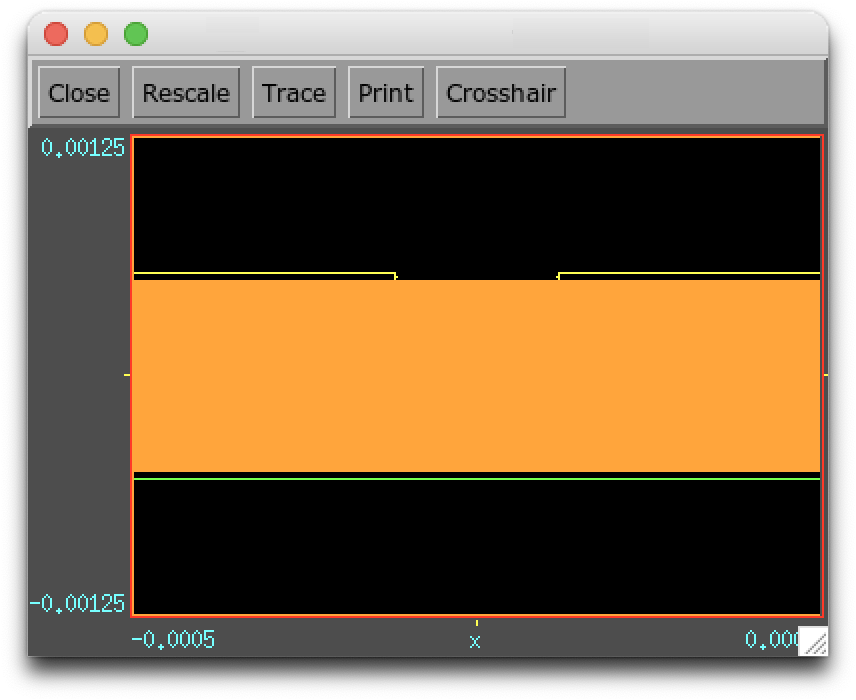
\includegraphics[width=0.9\linewidth]{chapter_4/figures/SRR_no_gap_start.png}
        \caption{}
        \label{fig:SRR_no_gap_start}
    \end{subfigure}%
    \begin{subfigure}{.5\textwidth}
        \centering
        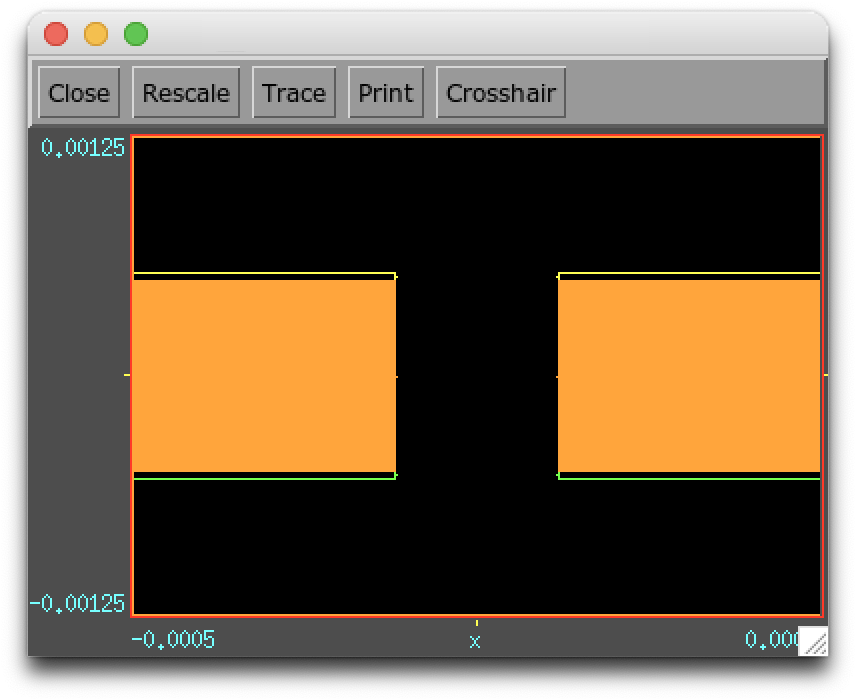
\includegraphics[width=0.9\linewidth]{chapter_4/figures/SRR_with_gap_start.png}
        \caption{}
        \label{fig:SRR_with_gap_start}
    \end{subfigure}
    \caption{A cross section comparison of SRR simulation domain without a hole (a) and with hole (b) in gap.}
    \label{fig:SRR_hole_comparison_start}
\end{figure}

The results of the simulation after it stabilised (which amounted to approximately 2 $\mu$s in simulation time) can be seen in figure \ref{fig:SRR_hole_comparison_stabilise}. The immediate difference that can be observed is the fact that the ions and electrons, represented as blue and orange dots respectively, tended to `sit' deeper into the gap in the case with the through hole. Intuitively, this would make sense as these particles are not colliding with the substrate. Additionally, it was hypothesised that strength of the electric field between the top electrodes and the ground plane could potentially play an effect in how deep the ions and electrons penetrate in the gap, which is investigated later.

\begin{figure*}[h!]
    \centering
    \begin{subfigure}[b]{0.475\textwidth}
        \centering
        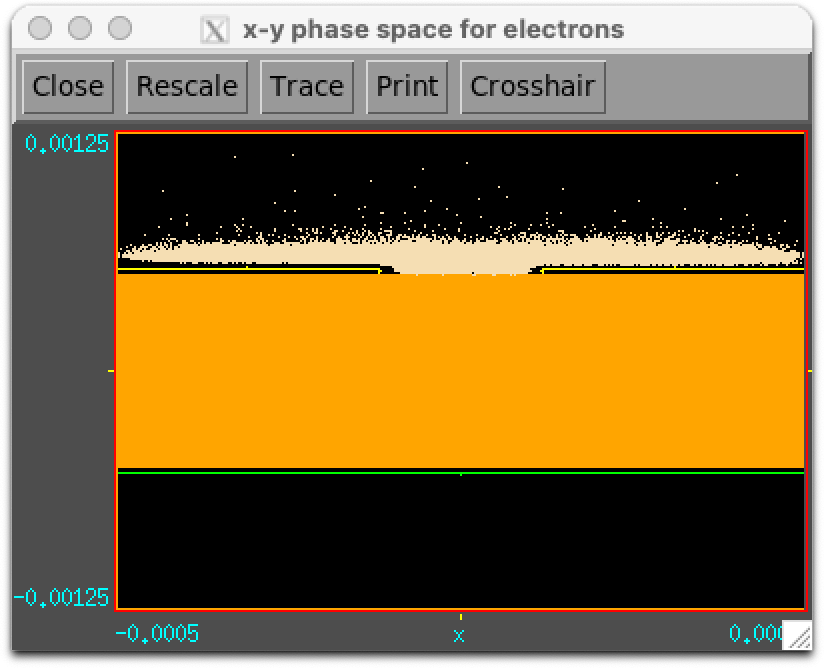
\includegraphics[width=\textwidth]{chapter_4/figures/SRR_no_hole_electrons.png}
        \caption{}
        \label{fig:SRR_no_hole_electrons}
    \end{subfigure}
    \hfill
    \begin{subfigure}[b]{0.475\textwidth}  
        \centering 
        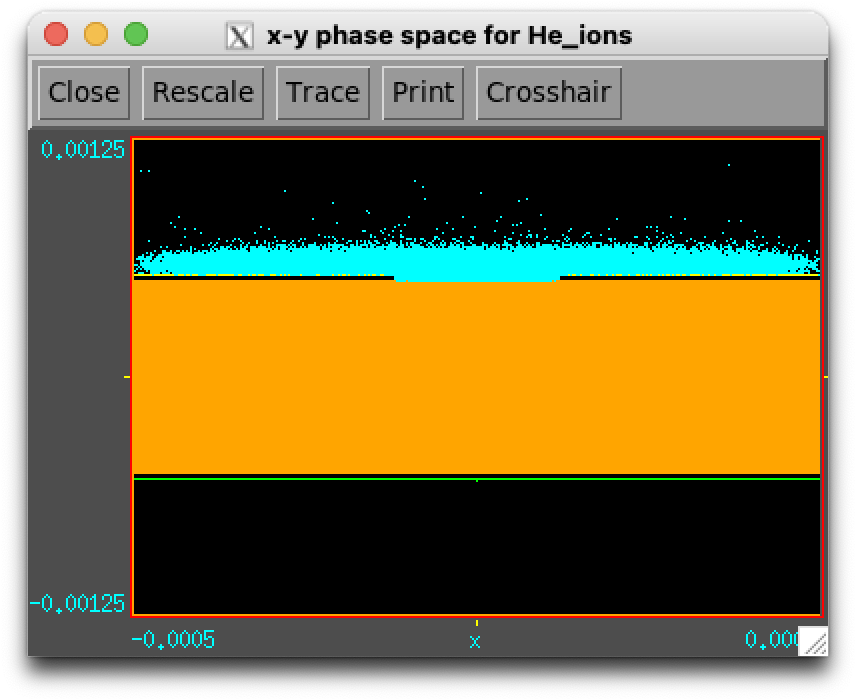
\includegraphics[width=\textwidth]{chapter_4/figures/SRR_no_hole_ions.png}
        \caption{}
        \label{fig:SRR_no_hole_ions}
    \end{subfigure}
    \vskip\baselineskip
    \begin{subfigure}[b]{0.475\textwidth}   
        \centering 
        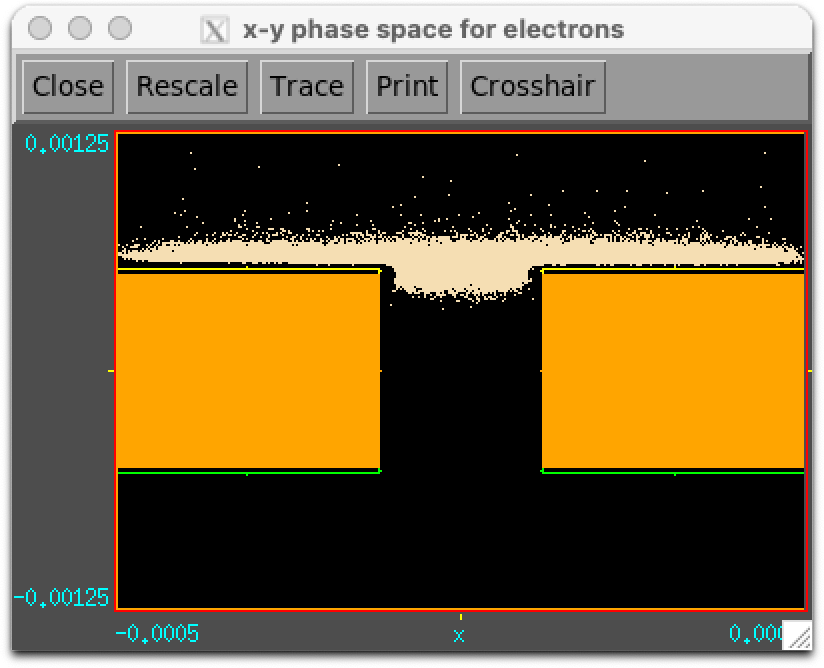
\includegraphics[width=\textwidth]{chapter_4/figures/SRR_with_hole_electrons.png}
        \caption{}
        \label{fig:SRR_with_hole_electrons}
    \end{subfigure}
    \hfill
    \begin{subfigure}[b]{0.475\textwidth}   
        \centering 
        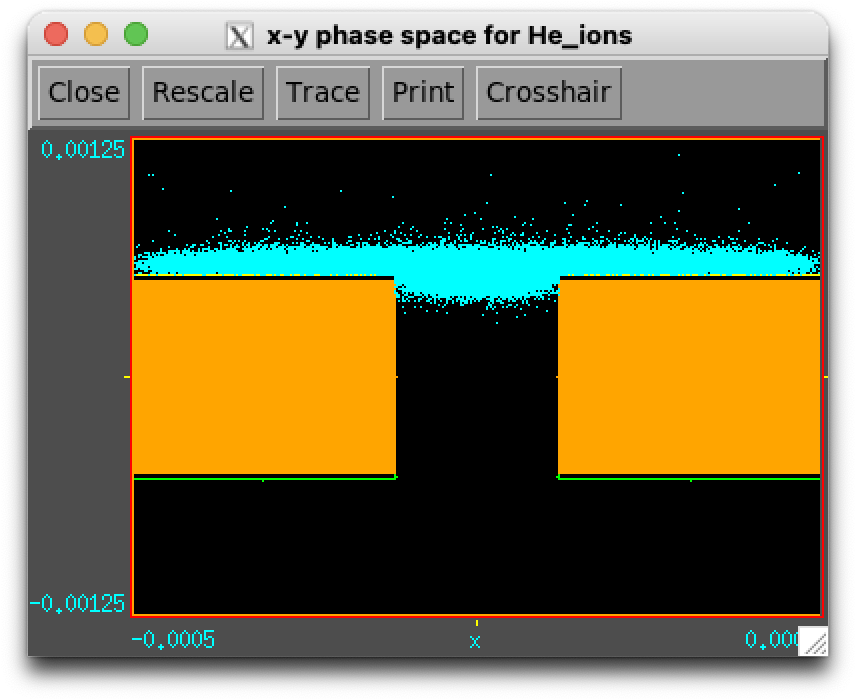
\includegraphics[width=\textwidth]{chapter_4/figures/SRR_with_hole_ions.png}
        \caption{}
        \label{fig:SRR_with_hole_ions}
    \end{subfigure}
    \caption[]
    {\small A comparison of the distribution of electron (a, c) and ions (b, d) in the discharge of the SRR. The top two subfigures (a, b) show the distribution in an SRR with no hole, while the bottom two (c, d) show the distribution in an SRR with a hole in the gap. 
    
    Comparison of SRR with and without hole in gap.} 
    \label{fig:SRR_hole_comparison_stabilise}
\end{figure*}

The next set of simulations run were to identify the ideal width discharge gap to be used. As seen in Paschen's law, it is one of the parameters governs to breakdown voltage. Hence selecting the ideal gap width should allow for a lower operating power. In these simulations, the only parameter changed was the gap width, taking the values of 120 $\mu$m, 180 $\mu$m, 240 $\mu$m, 300 $\mu$m, 360 $\mu$m, 420 $\mu$m, and 480 $\mu$m. 

Rather than observing the steady state characteristics, in these simulations the focus was to obtain the exact breakdown voltage for each gap, forming a very rough Paschen curve. To do this in simulations, one observes if a given voltage creates the Townsend avalanche resulting in the increase in the number of electrons in the simulation. This is better explained visually as shown in figures \ref{fig:SRR_gap_ignition_comparison}. 

\begin{figure}[h!]
    \centering
    \begin{subfigure}{0.7\textwidth}
        \centering
        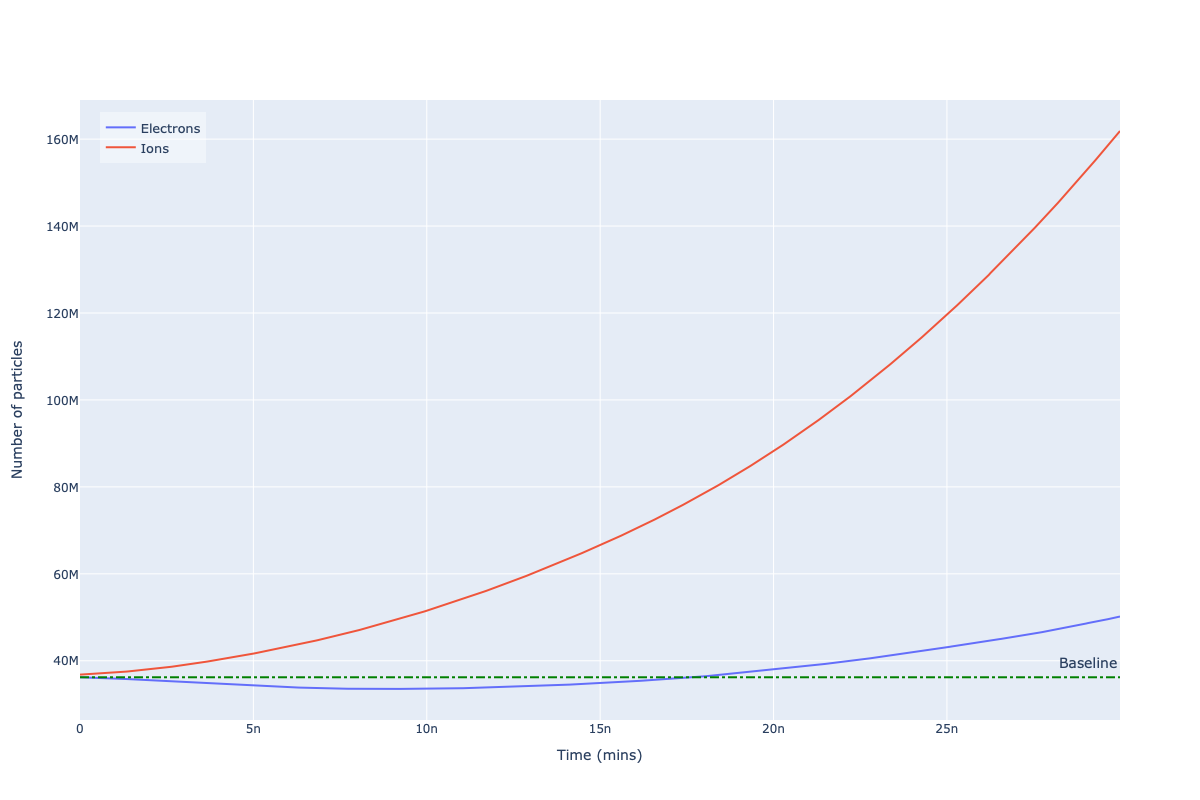
\includegraphics[width=0.9\linewidth]{chapter_4/figures/gap_test_ignition.png}
        \caption{}
        \label{fig:gap_test_ignition}
    \end{subfigure}%
    \vskip\baselineskip
    \begin{subfigure}{0.7\textwidth}
        \centering
        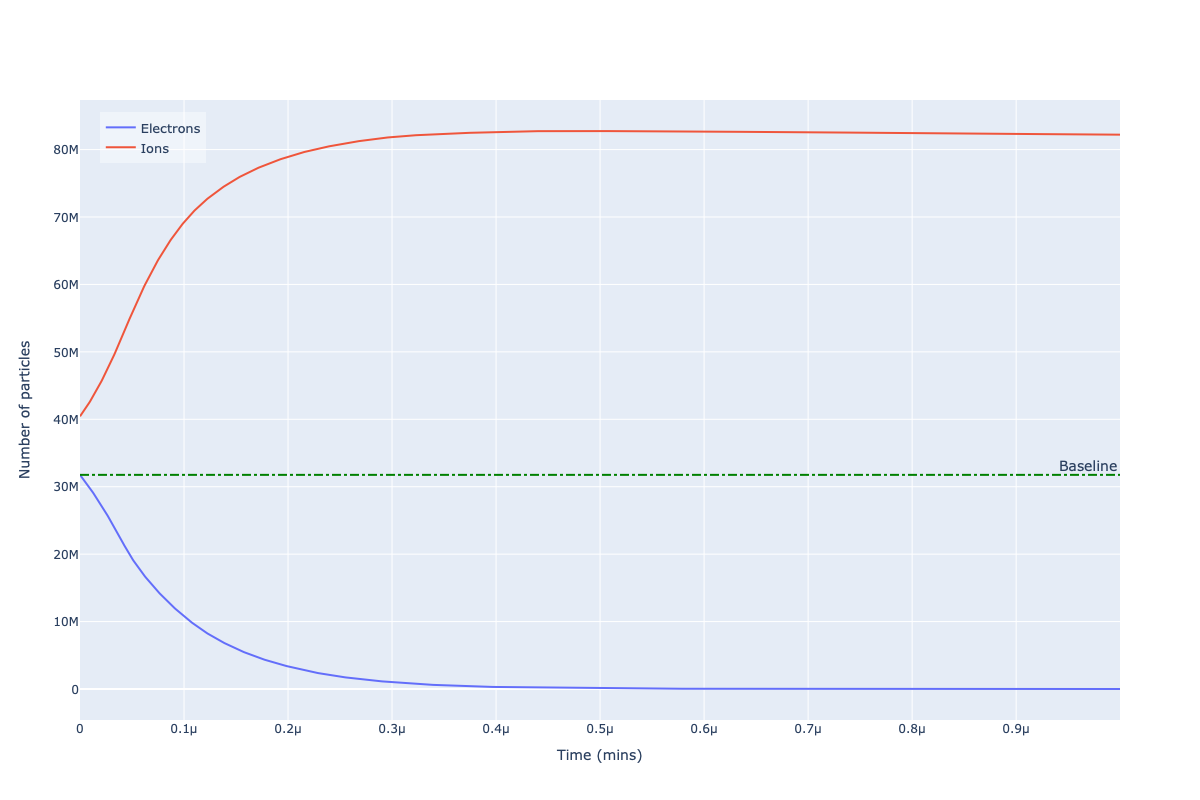
\includegraphics[width=0.9\linewidth]{chapter_4/figures/gap_test_no_ignition.png}
        \caption{}
        \label{fig:gap_test_no_ignition}
    \end{subfigure}
    \caption{A comparison of the number of particles diagnostic between a simulation potential difference of 150V (a) causing a voltage breakdown and one with a potential difference of 100V (b) which does not cause a breakdown.}
    \label{fig:SRR_gap_ignition_comparison}
\end{figure}

In figure \ref{fig:gap_test_ignition}, the number of electrons initially drop below the baseline but then increases again, meaning that the Townsend avalanche occurred, hence the plasma is said to be ignited. Whereas in figure \ref{fig:gap_test_no_ignition}, the number of electrons decreases until it reaches zero, meaning that the voltage set was not sufficient to cause a breakdown. The reason for the baseline number of electrons is due to seeding the simulations with particles.

This process of varying the simulation voltage was done across all the aforementioned gap widths to form a voltage breakdown curve shown in figure \ref{fig:gap_widths_breakdown_voltage}. From the data, it can be seen that the ideal gap width for the simulated design of the SRR was a 180$\mu$m discharge gap. However based on the shape of a Paschen curve, a smaller discharge gap  could be more optimal, though the gains would probably be marginal.

\begin{figure}[h!]
	\centering
	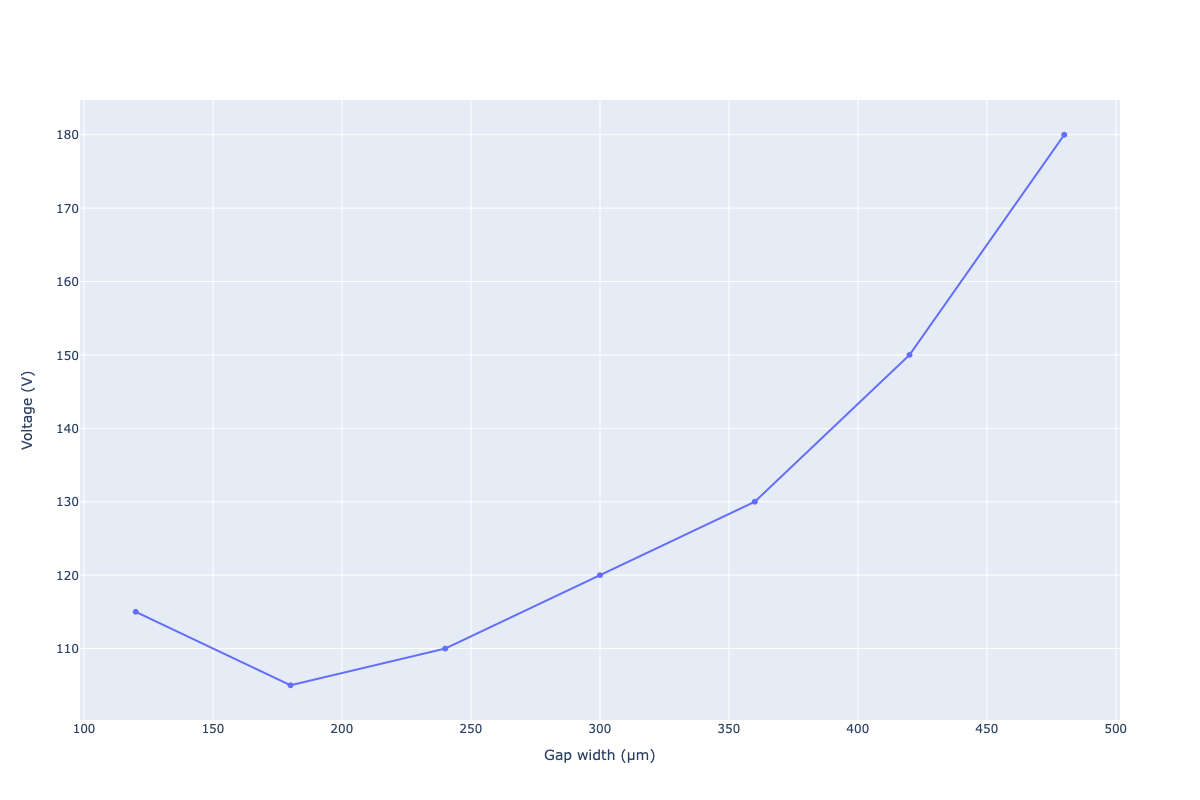
\includegraphics[width=0.7\linewidth]{chapter_4/figures/gap_widths_breakdown_voltage.png}
	\caption{Simulation breakdown voltages across the various tested discharge gap widths.}
	\label{fig:gap_widths_breakdown_voltage}
\end{figure}

With the optimal gap width identified, another parameter that needed to be looked into for the design of the SRR was the separation distance between the top and bottom electrodes. In other terms, it was to identify the ideal dielectric substrate thickness to be used when manufacturing the SRR. These simulations were split into two parts.

For the first part of the simulations regarding the dielectric thickness, the goal was to observe if changing the thickness would have any effect on the plasma behaviour. For these simulations, the dielectric thickness used were 0.2 mm, 0.5 mm, 1.0 mm, 1.5 mm, and 2.0 mm. The simulations were run until they stabilised, again to around 2 $\mu$s in simulation time. The results of these simulations can be seen in \ref{fig:SRR_dielectric_comparison_stabilise} in the form of a cross sectional view of the density plot of electrons. From the data, it can be seen that there are `hotspots' of electrons near the top electrons that vary from tests, however the overall density and shape of the plasma are almost identical. This implies that changing the dielectric thickness does not play a large role in the plasma behaviour, so other factors would need to be used to determine which dielectric thickness would be chosen for manufacturing the SRR.

\begin{figure*}[h!]
    \centering
    \begin{subfigure}[b]{0.475\textwidth}
        \centering
        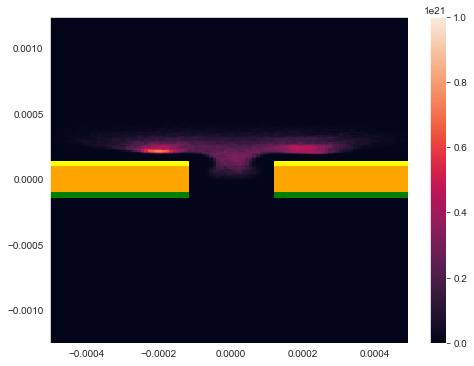
\includegraphics[width=\textwidth]{chapter_4/figures/SRR_dielectric_1.png}
        \caption{}  
        \label{fig:SRR_dielectric_0.2mm}
    \end{subfigure}
    \hfill
    \begin{subfigure}[b]{0.475\textwidth}  
        \centering 
        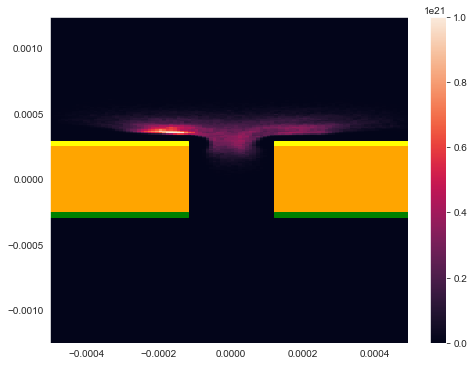
\includegraphics[width=\textwidth]{chapter_4/figures/SRR_dielectric_2.png}
        \caption{}   
        \label{fig:SRR_dielectric_0.5mm}
    \end{subfigure}
    \vskip\baselineskip
    \begin{subfigure}[b]{0.475\textwidth}   
        \centering 
        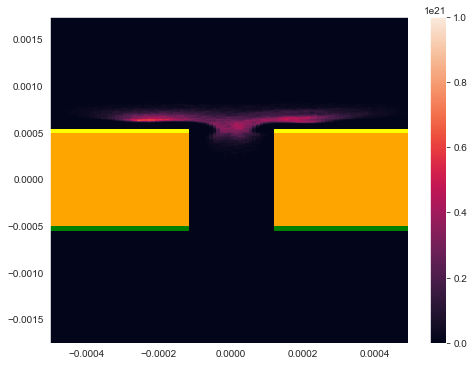
\includegraphics[width=\textwidth]{chapter_4/figures/SRR_dielectric_3.png}
        \caption{}    
        \label{fig:SRR_dielectric_1.0mm}
    \end{subfigure}
    \hfill
    \begin{subfigure}[b]{0.475\textwidth}   
        \centering 
        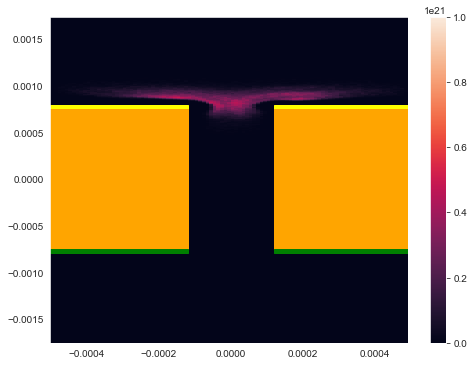
\includegraphics[width=\textwidth]{chapter_4/figures/SRR_dielectric_4.png}
        \caption{}   
        \label{fig:SRR_dielectric_1.5mm}
    \end{subfigure}
    \vskip\baselineskip
    \begin{subfigure}[b]{0.475\textwidth}   
        \centering 
        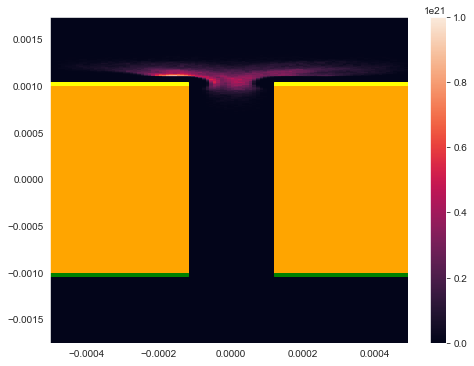
\includegraphics[width=\textwidth]{chapter_4/figures/SRR_dielectric_5.png}
        \caption{}    
        \label{fig:SRR_dielectric_2.0mm}
    \end{subfigure}
    \caption[]
    {\small Comparison of dielectric thickness of 0.2 mm (a), 0.5 mm (b), 1.0 mm (c), 1.5 mm (d), and 2.0 mm (e) on the SRR.} 
    \label{fig:SRR_dielectric_comparison_stabilise}
\end{figure*}


The first was to observe if increasing the dielectric thickness had any effect on the plasma characteristics, notably deep the plasma `sits' in the discharge gap. The other characteristic investigated was if changing the dielectric thickness would have any affect on the 

The other part of the dielectric thickness simulations was to identify if the thickness chosen would have an impact on the breakdown voltage since reducing the thickness would make the strength of the electric fields between the top electrodes comparable to the electric field between the AC electrodes and the ground plane. A similar approach was taken to simulations run for evaluating the impact of the gap width on breakdown voltage, though in this case the gap width was kept fixed and the only parameter changed was the thickness of the dielectric. The same values were used for the dielectric thickness as before.


The results for these simulations are shown in table \ref{}. TODO.
%TODO: run simulations on the dielectric thickness and breakdown voltage



\pagebreak


%This leads into the second group of simulations that were run, where the separation distance between the top and bottom electrodes were investigated, which also had the added benefit of identifying  the ideal dielectric substrate thickness to be used when manufacturing the SRR. The parameters used for the size of the gap, the dielectric constant of the substrate, and the potential difference were kept the same as the first group. As for the dielectric thickness, simulations were run with values of 0.2 mm, 0.5 mm, 1.0 mm, 1.5 mm, and 2.0 mm. 
%
%From the cross sectional view of the density plot of electrons in figure \ref{fig:SRR_dielectric_comparison_stabilise}, all simulations performed quite similarly. The electrons seem to extend through the gap by roughly the same distance. However, even though the dielectric thickness did not play a large role in the plasma, it would be preferable to choose a thicker dielectric for the sturdiness of the board. 
%
%The final group of simulations run were to establish the effect of the discharge gap widths. The sizes used were a gap width of 120 $\mu$m, 240 $\mu$m, 360 $\mu$m, and 480 $\mu$m. 
%
%\begin{figure}[h!]
%	\centering
%	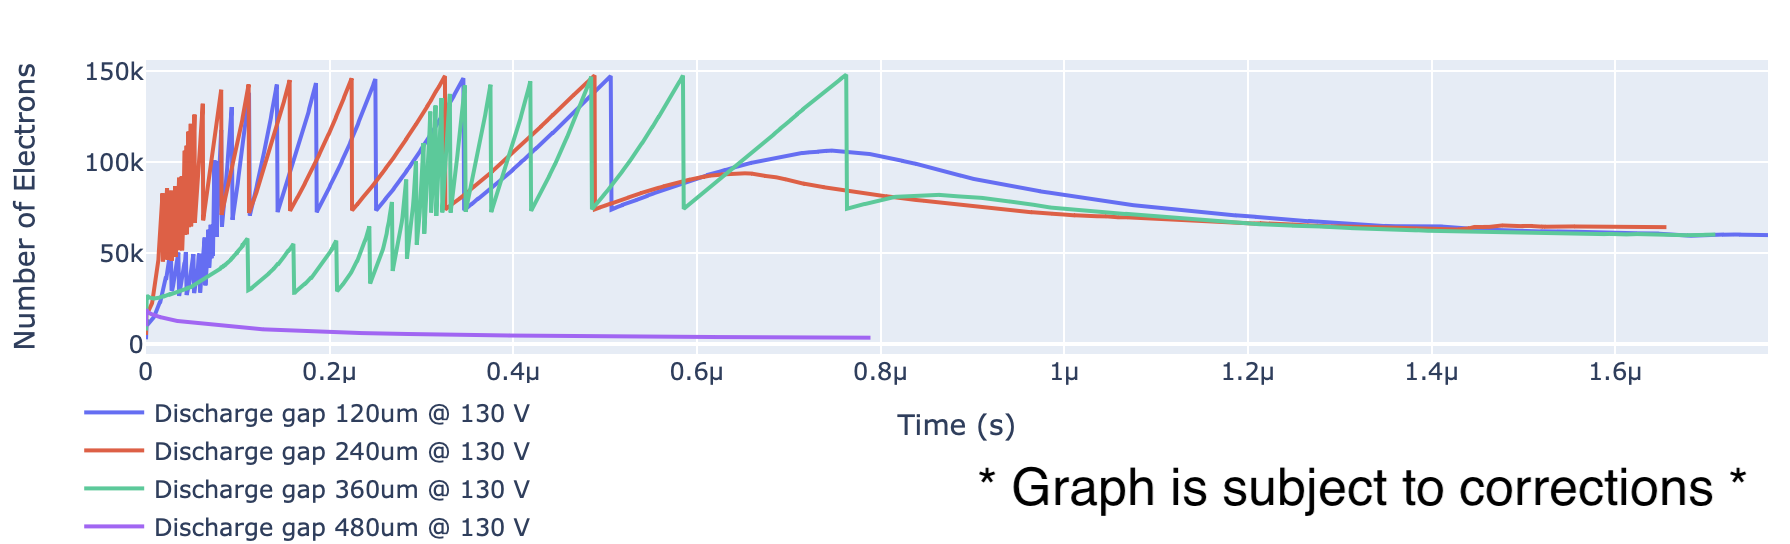
\includegraphics[width=\linewidth]{chapter_4/figures/num_elec_gap.png}
%	\caption{Time series plot of number of electrons across different discharge gaps.}
%	\label{fig:num_elec_gap}
%\end{figure}
%
%The results of these simulations can be seen in figure \ref{fig:num_elec_gap}. From these tests, only three simulations were successful as the run with a gap width of 480 $\mu$m lost all the electrons. The reasons for this behaviour was that the voltage used (150 V) was not sufficient to ignite a discharge, as the electric field in the gap reduces with an increase in gap width. As for the other three runs, the big difference seemed to be the initial growth rate. A gap width of 240 $\mu$m appeared to be the optimum. One would expect that the smallest gap width would perform the best, however as seen by Paschen's law (refer to Chapter \ref{sec:paschens_law}), reducing the distance between electrodes too much would cause the electrons to be simply lost to the electrode. This could possibly explain why the run with a 120 $\mu$m gap performed worse than the run with a gap width of 240 $\mu$m.



\subsection{Design}

Using the results from the simulations run, a design of the SRR to be used could be made. The first step was to selected the desired operating frequency (also referred to as the resonant frequency). Selecting this frequency for the SRR required striking a compromise. Ideally, a higher resonant frequency would improve the quality factor, reducing power losses and making it more likely that a plasma discharge occurs. However, a frequency that is too high would increase power requirements required to drive the SRR. An additional drawback to using higher frequencies is that as seen in equation \ref{eq:resonant_frequency}, increasing the frequency causes a decrease in the wavelength, which in turn reduces the size of the SRR. While this is not directly a problem, a smaller ring for the SSR would require significantly tighter manufacturing tolerances which in turn drive up the cost of production. As such, a target frequency of 1 GHz was chosen to strike a balance between the these factors. 


The next step was to then select the PCB substrate to be used, as its dielectric constant ($\varepsilon_r$) is another central parameter for all other calculations of the SRR. For this, the material selected was the RO4350B\textsuperscript{TM} substrate from Rogers corporation. This material was chosen over traditional PCB substrates, such as FR4, due to its excellent dissipation factor (D$_f$) at high frequencies. RO4350B\textsuperscript{TM} had a D$_f = 0.0031$ (at 2.5 GHz) whereas FR4 had a D$_f = 0.022$ (at 500 MHz). Though not an apples to apples comparison, the D$_f$ typically increases with frequency. Thus at approximately 1 GHz, the D$_f$ for FR4 would be an order of magnitude over that of the RO4350B\textsuperscript{TM} substrate. In the real world, this translates to a higher insertion loss for FR4 over RO4350B\textsuperscript{TM}, resulting in worse efficiency. Though better performing substrates were available, they came with the tradeoff of manufacturing cost, hence using RO4350B\textsuperscript{TM} was a suitable compromise. Additionally, RO4350B\textsuperscript{TM} did not require any special treatments or procedures to introduce a through hole.

According to its data sheet, the RO4350B\textsuperscript{TM} board has a dielectric constant ($\varepsilon_r$) of 3.66. However, the data sheet also specified that this result was only tested for the frequencies between 8 to 40 GHz; significantly higher than the desired operating frequency. From a previous experiment operating at roughly 500 MHz, it was ascertained that the $\varepsilon_r$ was reduced by nearly 25\% compared to the stated value, giving a $\varepsilon_r = 2.93$. Thus, this was the assumed value of the $\varepsilon_r$ when designing the SRR.

Feeding the target resonant frequency and $\varepsilon_r$ into equation \ref{eq:resonant_frequency}, gives a the wavelength of 0.175 m. ince the circumference of the SRR is given as $\lambda/2$, this meant that the design had a circumference of 8.7 cm; which gives the SRR a radius of approximately 1.385 cm. 

With the circumference of the ring determined, the next step was to set the parameters that determine the devices characteristic impedance. Again, this value should be as close to the input impedance of 50 $\Omega$. As stated previously, the characteristic impedance is governed by four factors, but the most important factor when determining the design requirements of the SRR was the thickness of the dielectric substrate. From the simulations, there was no difference in the plasma behaviour between different substrate thicknesses, but from a mechanical standpoint, a thicker substate would be preferable for structural rigidity. The only issue with this is that a thicker substrate comes with the detriment of additional manufacturing cost. Hence a dielectric substrate thickness of 0.5 mm was selected. 

With the substrate thickness and $\varepsilon_r$ selected, and the thickness of the copper pour being fixed by the manufacture (at 35 $\mu$m), the final step was to tune the width of the ring to give an impedance of 50 $\Omega$. By using the equations \ref{eq:wheeler_microstrip}-\ref{eq:wheeler_effective_w}, a trace width of approximately 1.05 mm would produce a characteristic impedance of 50.1 $\Omega$.

%Armed with this information, a design of the SRR to be used was made. The first step was to select the PCB substrate to be used, as its dielectric constant is a central parameter for all other calculations of the SRR. The material selected was the RO4350B\textsuperscript{TM} material from Rogers corporation. This specific material was chosen as it is designed for high power UHF designs, and its relatively low fabrication costs. Additionally, the RO4350B\textsuperscript{TM} material did not require any special treatments or procedures to introduce a through hole. According to its data sheet, the RO4350B\textsuperscript{TM} board has a dielectric constant of 3.66, and a dissipation factor of 0.0031 (which can be converted to the quality factor). In the data sheet, these values were tested at a frequency of 2.5 GHz. However, an assumption was made during the design process that these values would be approximately equivalent for the operational frequency selected.  
%
%Choosing the resonant frequency for the SRR required striking a compromise. Ideally, a higher resonant frequency would improve the quality factor, reducing power losses and making it more likely that a plasma discharge occurs. However, a frequency that is too high would increase power requirements required to drive the SRR. An additional drawback to using higher frequencies is that as seen in equation \ref{eq:resonant_frequency}, increasing the frequency causes a decrease in the wavelength, which in turn reduces the size of the SRR. While this is not directly a problem, a smaller ring for the SSR would require significantly tighter manufacturing tolerances which in turn drive up the cost of production. Therefore, a target frequency of 500 MHz was chosen to strike a balance between the these factors. 
%
%Feeding this number into equation \ref{eq:resonant_frequency}, the corresponding wavelength was 0.314 m. Since the circumference of the SRR is given as $\lambda/2$, this meant that the design had a circumference of 15.71 cm; which gives the SRR a radius of approximately 2.5 cm. 

%The next step was to determine the characteristic impedance. Conventionally, this impedance should be close to the value of the input impedance, which for power supply used was 50 $\Omega$. As mentioned earlier in this chapter, three factors dictate the value of this parameter. The dielectric constant of the substrate was 3.66, a fixed value based on the material used. As stated in the previous section, a thicker dielectric substate would be preferable. The RO4350B\textsuperscript{TM} material came in a thickness of 0.5 mm, 0.8 mm, and 1.55 mm; with the costs increasing with thickness. Thus, as a compromise between the structural rigidity PCB and cost, a thickness of 0.8 mm was selected. By using the equations \ref{eq:wheeler_microstrip}-\ref{eq:wheeler_effective_w}, a trace width of approximately 1.7 mm would produce a characteristic impedance of 50.1 $\Omega$.

Finally using equation \ref{eq:offset_angle}, the offset angle of the SRR was calculated. As from the datasheet, the dissipation factor of the RO4350B\textsuperscript{TM} material is 0.0031. The reciprocal of this value was taken to determine the quality factor, which was 323. This would give a gap with an offset angle of 7.99. Again based on the simulations above, the ideal gap width was 180 $\mu$m, however the minimum size drill hole size would be the limiting factor when manufacturing the device, hence the gap width was slightly increased to 250 $\mu$m. Though from the simulations, the gap width of 240 $\mu$m only increased the breakdown voltage by around 5\%.

With these parameters known, the next stage was to create the PCB design. This was done using the open-sourced PCB design software called \textit{KiCad}\footnote{https://www.kicad.org}. One benefit of using KiCad was the output files were natively supported by  the PCB manufacturer used, \textit{EuroCircuits}\footnote{https://www.eurocircuits.com}. 

An illustration of the final design can be seen in figure \ref{fig:SRR_cad}. As seen from the figure, four SRR designs were made. These were done to test various gap designs that could not be replicated using XOOPIC simulations. These designs could be broken down into two categories: single versus multiple drill hole in the SRR gap; and the presence versus absence of `finger-like' copper pours next to the SRR gap. The permutations of these categories resulted in the four designs, with a close up image of each shown in figure \ref{fig:SRR_cad_close_up}. All four designs used an SMA connector as the input source. 

\begin{figure}[h!]
	\centering
	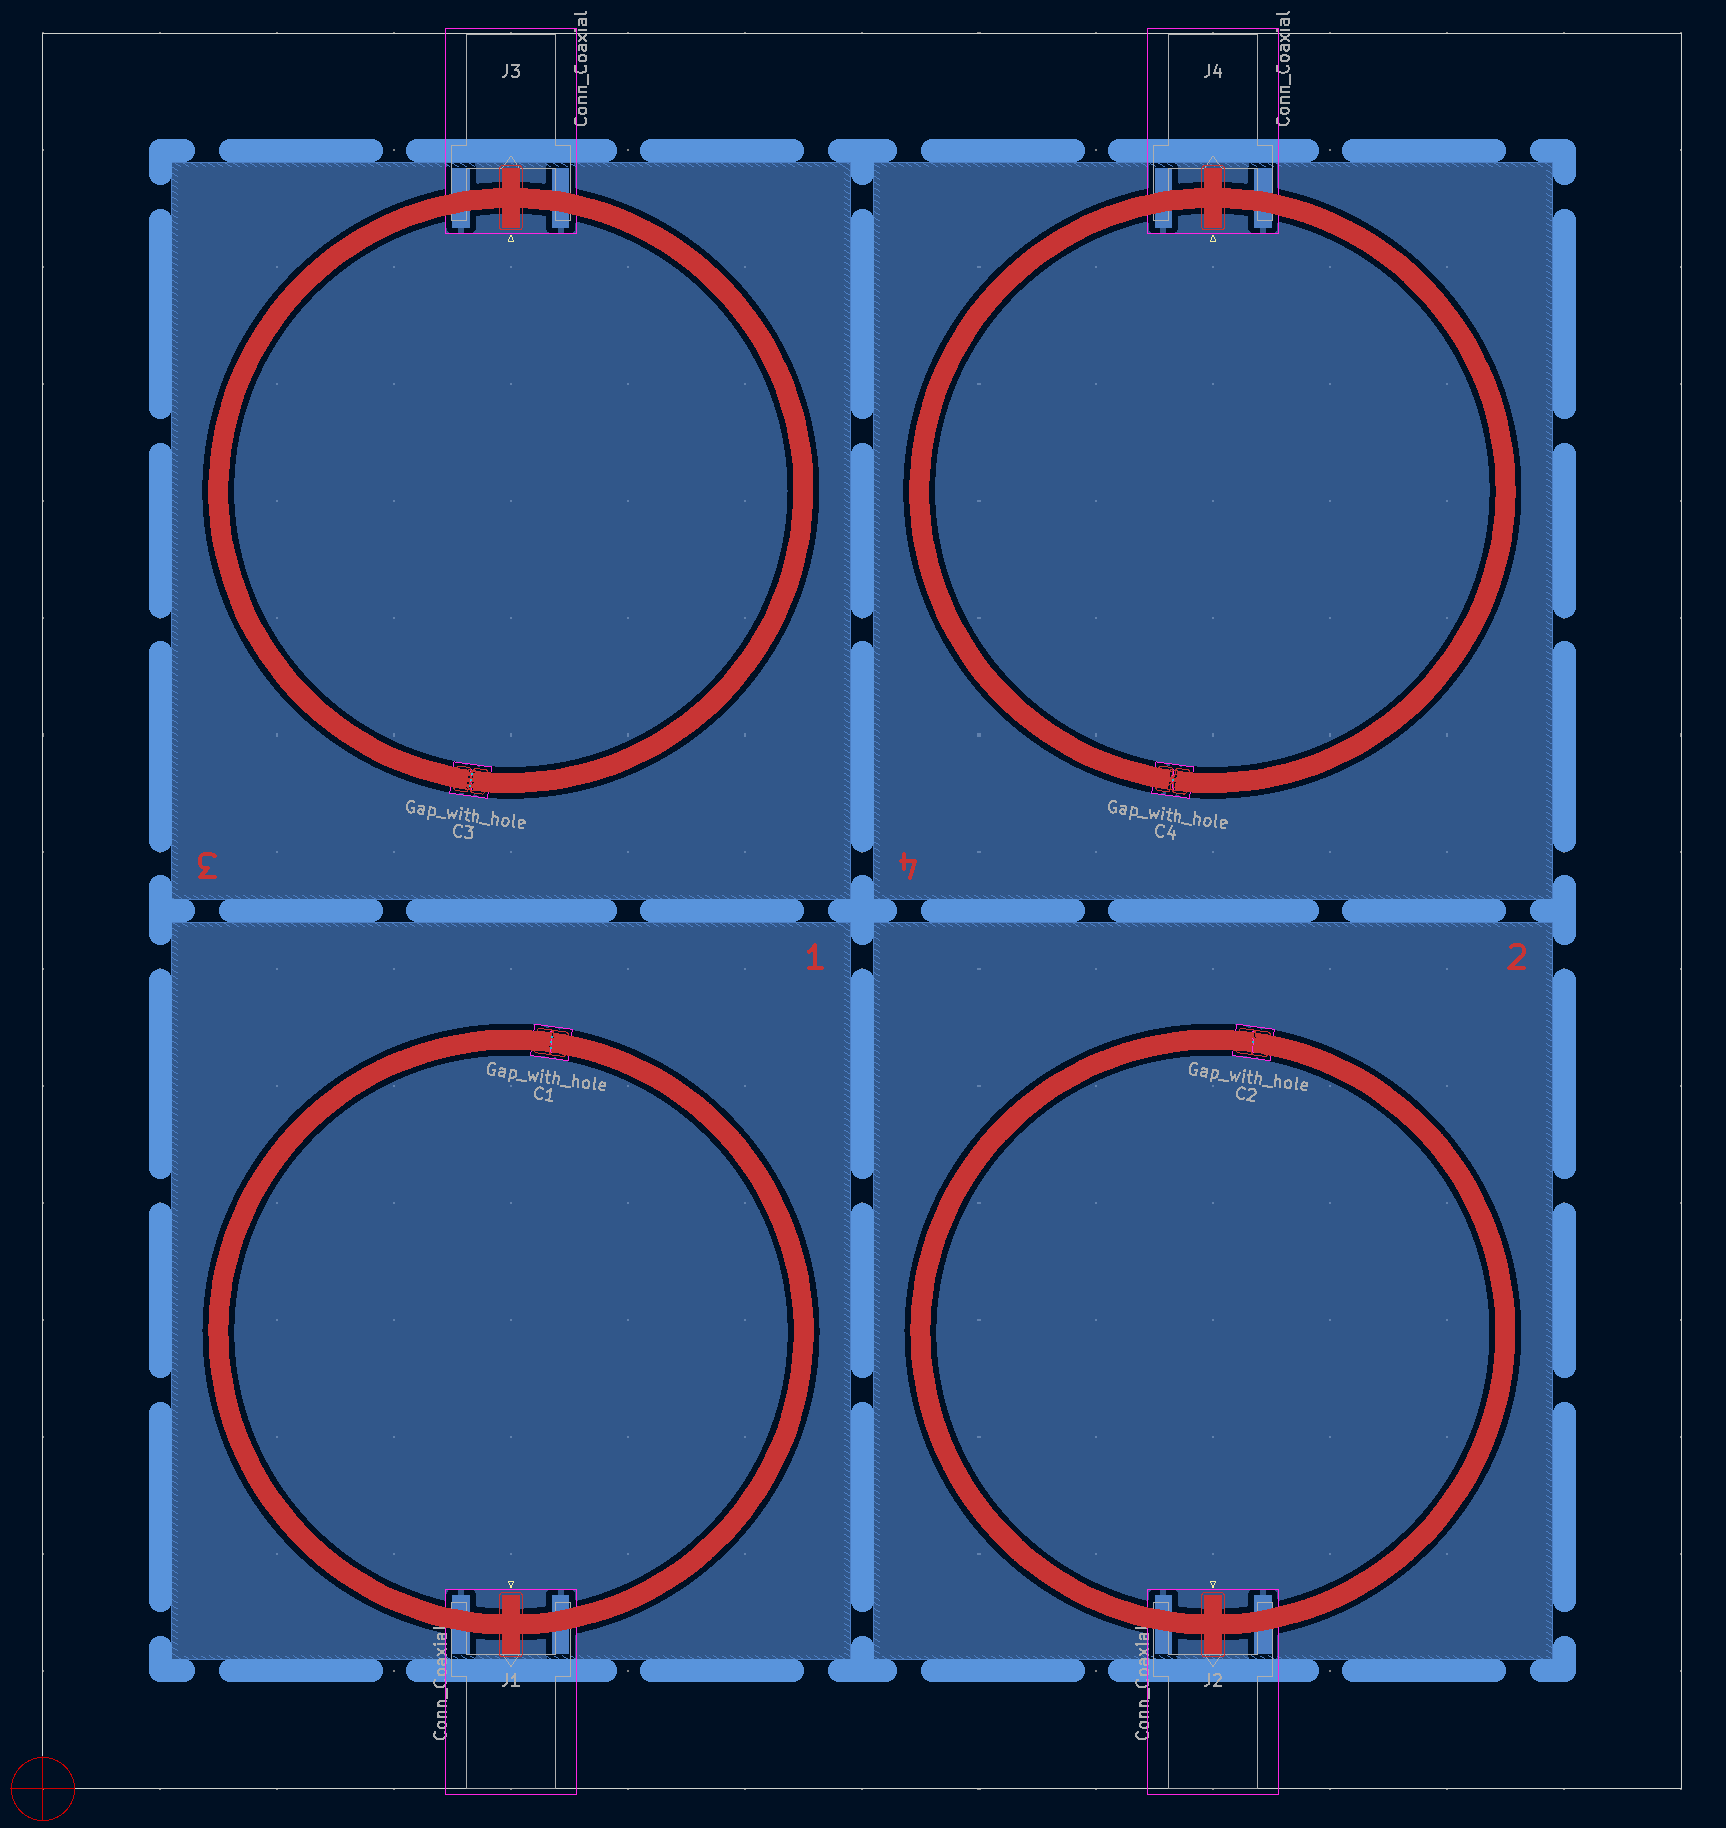
\includegraphics[width=0.8\linewidth]{chapter_4/figures/SRR_CAD.png}
	\caption{PCB schematic of SRR panels in the KiCad software suite.}
	\label{fig:SRR_cad}
\end{figure}

\begin{figure}
    \centering
    \begin{subfigure}[b]{0.475\textwidth}
        \centering
        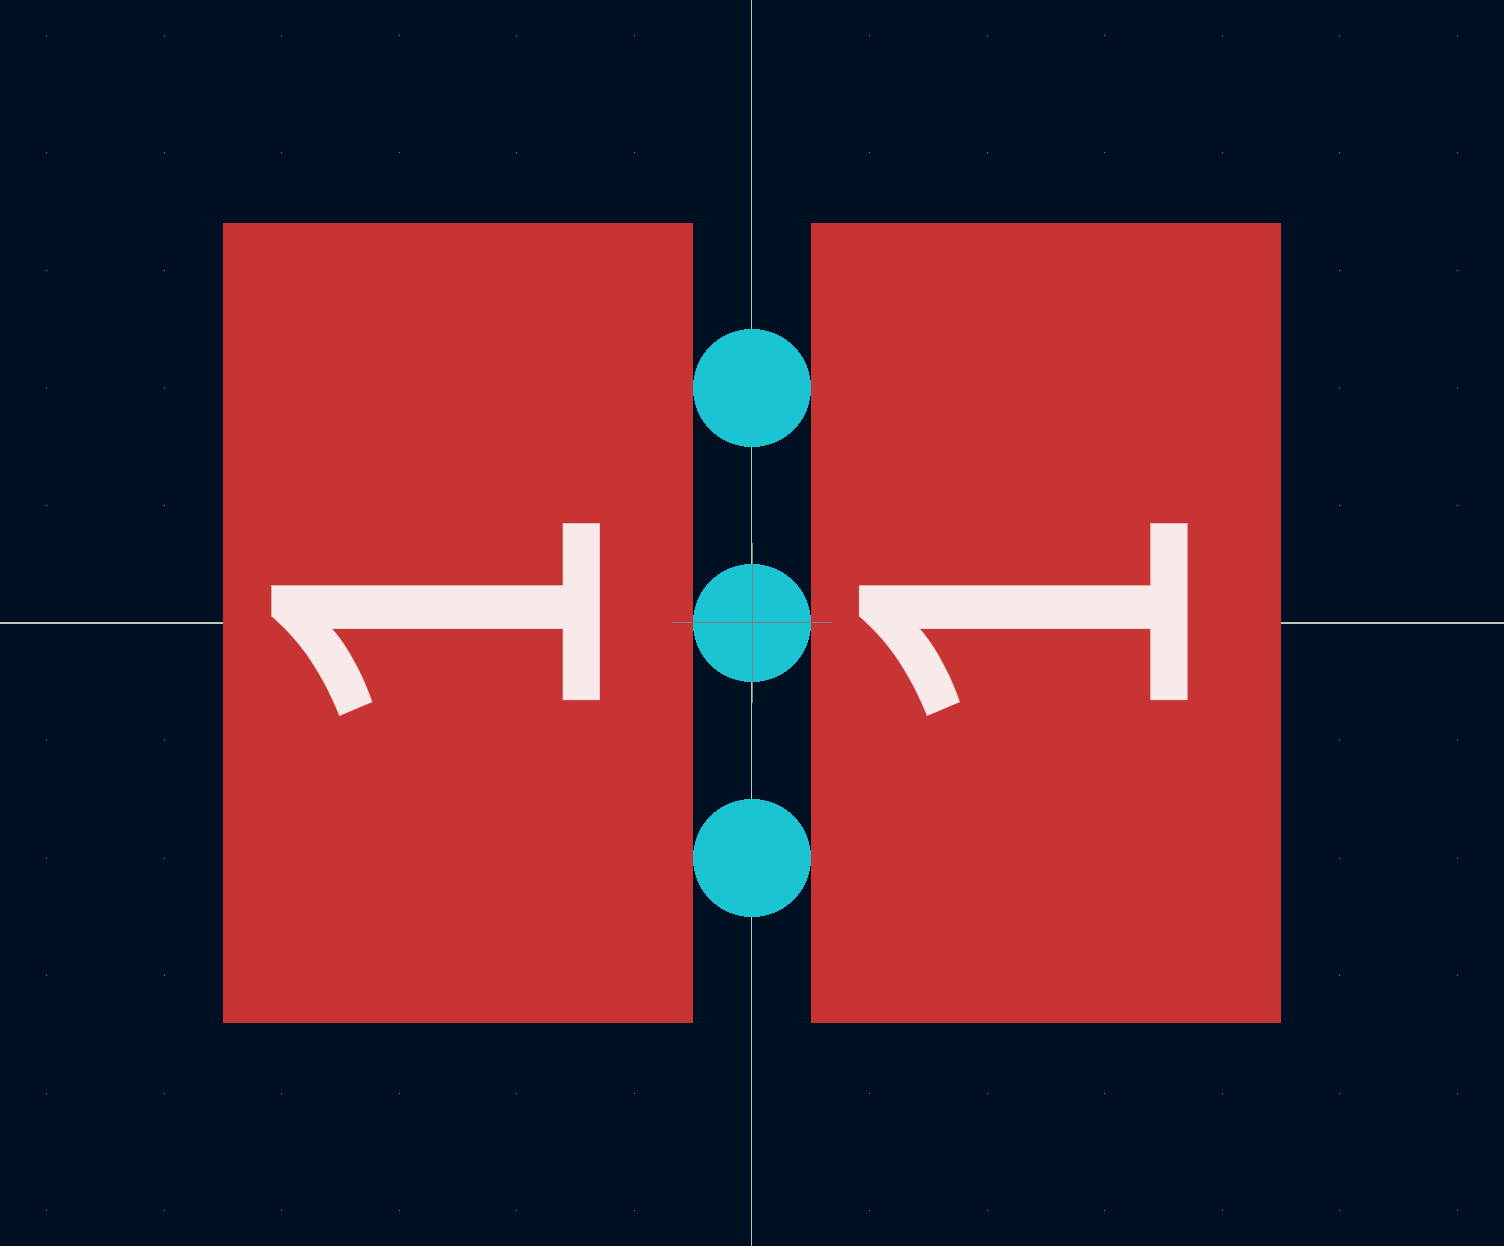
\includegraphics[width=\textwidth]{chapter_4/figures/SRR_CAD_hole_1.png}
        \caption{}
        \label{fig:design_1}
    \end{subfigure}
    \hfill
    \begin{subfigure}[b]{0.475\textwidth}  
        \centering 
        
\includegraphics[width=\textwidth]{chapter_4/figures/SRR_CAD_hole_2.png}
        \caption{}
        \label{fig:design_2}
    \end{subfigure}
    \vskip\baselineskip
    \begin{subfigure}[b]{0.475\textwidth}   
        \centering 
        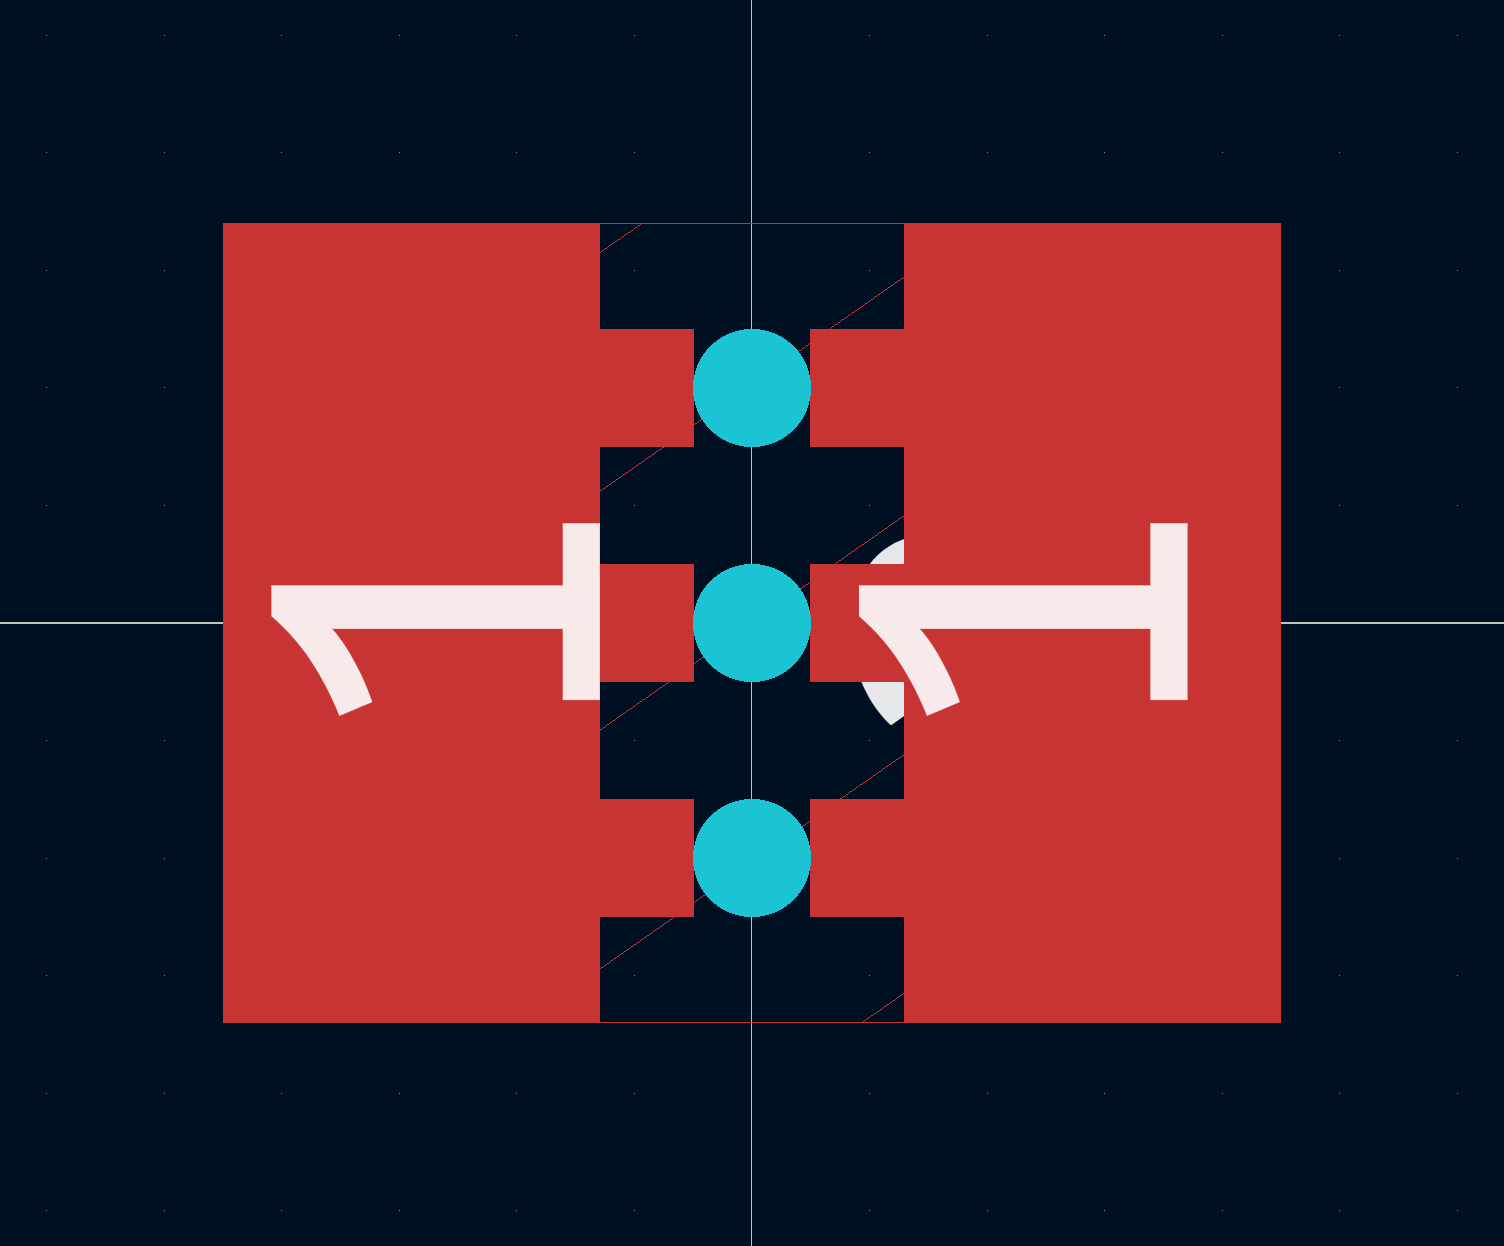
\includegraphics[width=\textwidth]{chapter_4/figures/SRR_CAD_hole_3.png}
        \caption{}
        \label{fig:design_3}
    \end{subfigure}
    \hfill
    \begin{subfigure}[b]{0.475\textwidth}   
        \centering 
        
\includegraphics[width=\textwidth]{chapter_4/figures/SRR_CAD_hole_4.png}
        \caption{}
        \label{fig:design_4}
    \end{subfigure}
    \caption{\small SRR gap designs with multiple holes (a, c) versus single holes (b, d). The designs in the lower two subfigures (c, d) have the presence of `finger-like' copper pours next to the holes.} 
    \label{fig:SRR_cad_close_up}
\end{figure}





%%\pagebreak
\section{Testing}
\subsection{Scattering Parameters}
%
%A picture of the manufactured SRR panel can be seen in figure \ref{}. The SMA connector attached is capable of delivering around 500 V, up to a frequency of 18 GHz; far beyond the capabilities of the SRR device.

The next step was to compare the real-world characteristics of the device to the theoretical calculations. The first of these tests was to evaluate the \textit{scattering parameters} (S-parameters) of the device. The S-parameters are a measurement of the linear characteristics of a device under test (DUT) such as its gain, impedance, and phase delay, as a function of frequency. This test is typical done on high-frequency RF or microwave circuits, ranging with one or more ports; with the results in the form of an $N \times N$ matrix, where $N$ is the number of ports on the DUT. Since the SRR has only a single port, its characteristics are given by a simple $1  \times  1$ matrix with the value $s_{11}$. As such, this $s_{11}$ parameter describes the ratio of the forward power going into the device and the reflected power coming out, and is governed by:
\begin{equation}
    s_{11} (dB) = -10 log (\frac{P_{forward}}{P_{reflected}}) 
\end{equation}

The $s_{11}$ characteristics of the SRR were measured using a vector network analyser (VNA), specifically the \textit{PicoVNA$^{\textregistered}$}. A sweep between 500 MHz to 1.5 GHz was performed. Since the SRR was designed to resonate at approximately 1 GHz, this should place a single largest peak at roughly the centre of the frequency range, and the broad range would also capture any shifts in the resonant frequency due to manufacturing tolerances. 

\begin{figure}[h!]
	\centering
	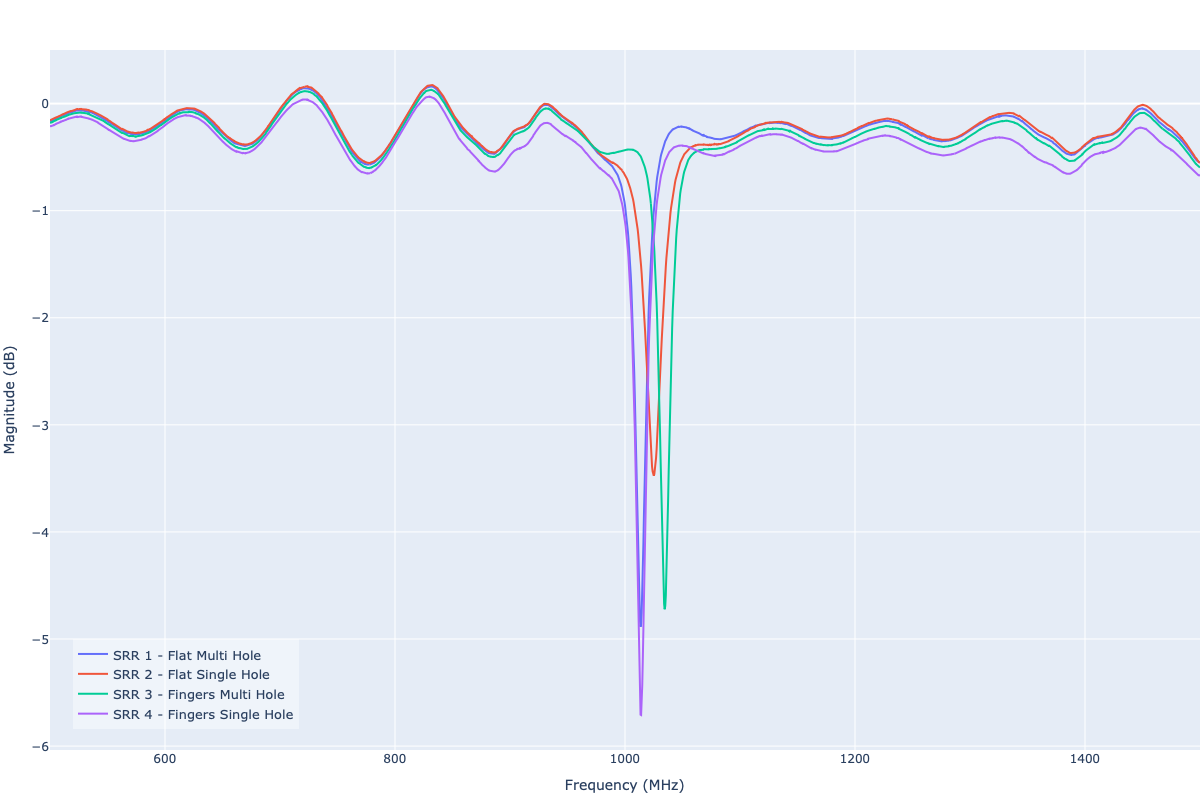
\includegraphics[width=\linewidth]{chapter_4/figures/S11.png}
	\caption{Reflection coefficient (S$_{11}$) of SRR in dB.}
	\label{fig:SRR_s11}
\end{figure}


Figure \ref{fig:SRR_s11} shows the results of the $s_{11}$ parameter tests for a sample of the four designs made, with the y-axis indicating the magnitude of attenuation (in decibels) at a given frequency. From the data, it is immediately obvious that for a given test, there was only one strong attenuation peak. The value of this peak varied from each board tested but they ranged from 1.01 to 1.03 GHz. This equated to an error of roughly 1-3\% from the designed resonant frequency, which would be inline with the margin of manufacturing tolerances and design assumptions. 

However, the magnitude of attenuation for the devices (i.e. from the depth of the peaks) were much lower than expected. The expected quality factor was in the order of $Q \approx 300$ but the quality factor attained was closer to $Q \approx 90$. This implies that the assumption made in the design phase regarding the dielectric constant and dissipation factor were incorrect. While this should not necessarily affect the ability of the device to ignite a plasma and sustain the discharge, it would do so at a higher power thus hurting the power efficiency of the device.


%From the data it is immediately obvious that there is only one peak at 1.02 GHz which would be inline with the margin of error for the designed resonant frequency. Though the depth of the peak shows that the real world device has a much lower quality factor. This implies that the assumption made in the design phase regarding the dielectric constant and dissipation factor were incorrect. While this does not necessarily affect the plasma discharge, it does mean that a higher power is going to be required to ignite the plasma.


%From the data, it is immediately obvious that there are two peaks, instead of the expected result which would be a single peak. The first of these peaks is at 554 MHz, which would be inline with the margin of error for the designed resonant frequency. The second peak on the other hand, located at approximately 753 MHz represents some additional resonance present in the SRR device. The source of this resonance could be either from the SMA connector itself, or from the design of the SRR, or both. Examples of areas of the design that could introduce resonance could be the overall dimension of the SRR panel or even the of gaps on the underside along the ground ring (a by-product of the design process). Nonetheless, this is just conjecture and the exact reasoning for the presence of this peak would be difficult to ascertain without going into high-frequency structure simulations which are beyond the scope of this project. While this second peak indicates a stronger resonance, as seen by the larger attenuation, it does not mean it is possible to ignite a plasma at that frequency. This is because the formation of the plasma is governed by the geometry of the SRR.
%
%As for first peak at 554 MHz, it appeared to have a much lower quality factor in the real world. This implies that the assumption made in the design phase regarding the dielectric constant and dissipation factor were incorrect. While this does not necessarily affect the plasma discharge, it does mean that a higher power is going to be required to ignite the plasma.

\subsection{Experimental Setup}

Once the true resonant frequency was determined, the next step was to setup the experiment. Note that this is not the final setup to be used for recirculating the gases, instead it was used to reliably ignite a plasma from the SRR in order to characterise it and understand its behaviour. An illustration of the setup is seen in figure \ref{fig:SRR_setup}.

\begin{figure}[h!]
	\centering
	\includegraphics[width=\linewidth]{chapter_4/figures/SRR_setup.png}
	\caption{Schematic of experimental setup.}
	\label{fig:SRR_setup}
\end{figure}

In the setup, there are two mass flow controllers by MKS Instruments. For the time being, these are only controlling the flow of helium gas into the setup; the introduction of carbon dioxide gas is discussed in the next chapter. The first one (MFC$_1$)  is positioned on the bottom side of the SRR, whilst the second one (MFC$_2$) controls the flow to the chamber. The reason for two separate mass flow controllers is that the size of the aperture of the SRR is quite small (with a diameter of 0.25 mm), hence only using one controller to pressurise the entire apparatus at 760 Torr (which is one atmosphere) would take a long time. Thus, MFC$_2$ is used to maintain pressure the pressure of the chamber whilst MFC$_1$ maintains a flow of Helium through the gap of the SRR. 

The SRR device is oriented so that the Helium flows from the bottom (i.e. the ground ring) to top; (i.e. the AC ring). This is because the plasma discharge occurs at the top of the ring, thus when used later in the epoxidation process, this is the side that is going to face the liquid co-reactant. A photograps of the plasma can be seen in figure \ref{fig:SRR_plasma}. 

\begin{figure}[h!]
	\centering
	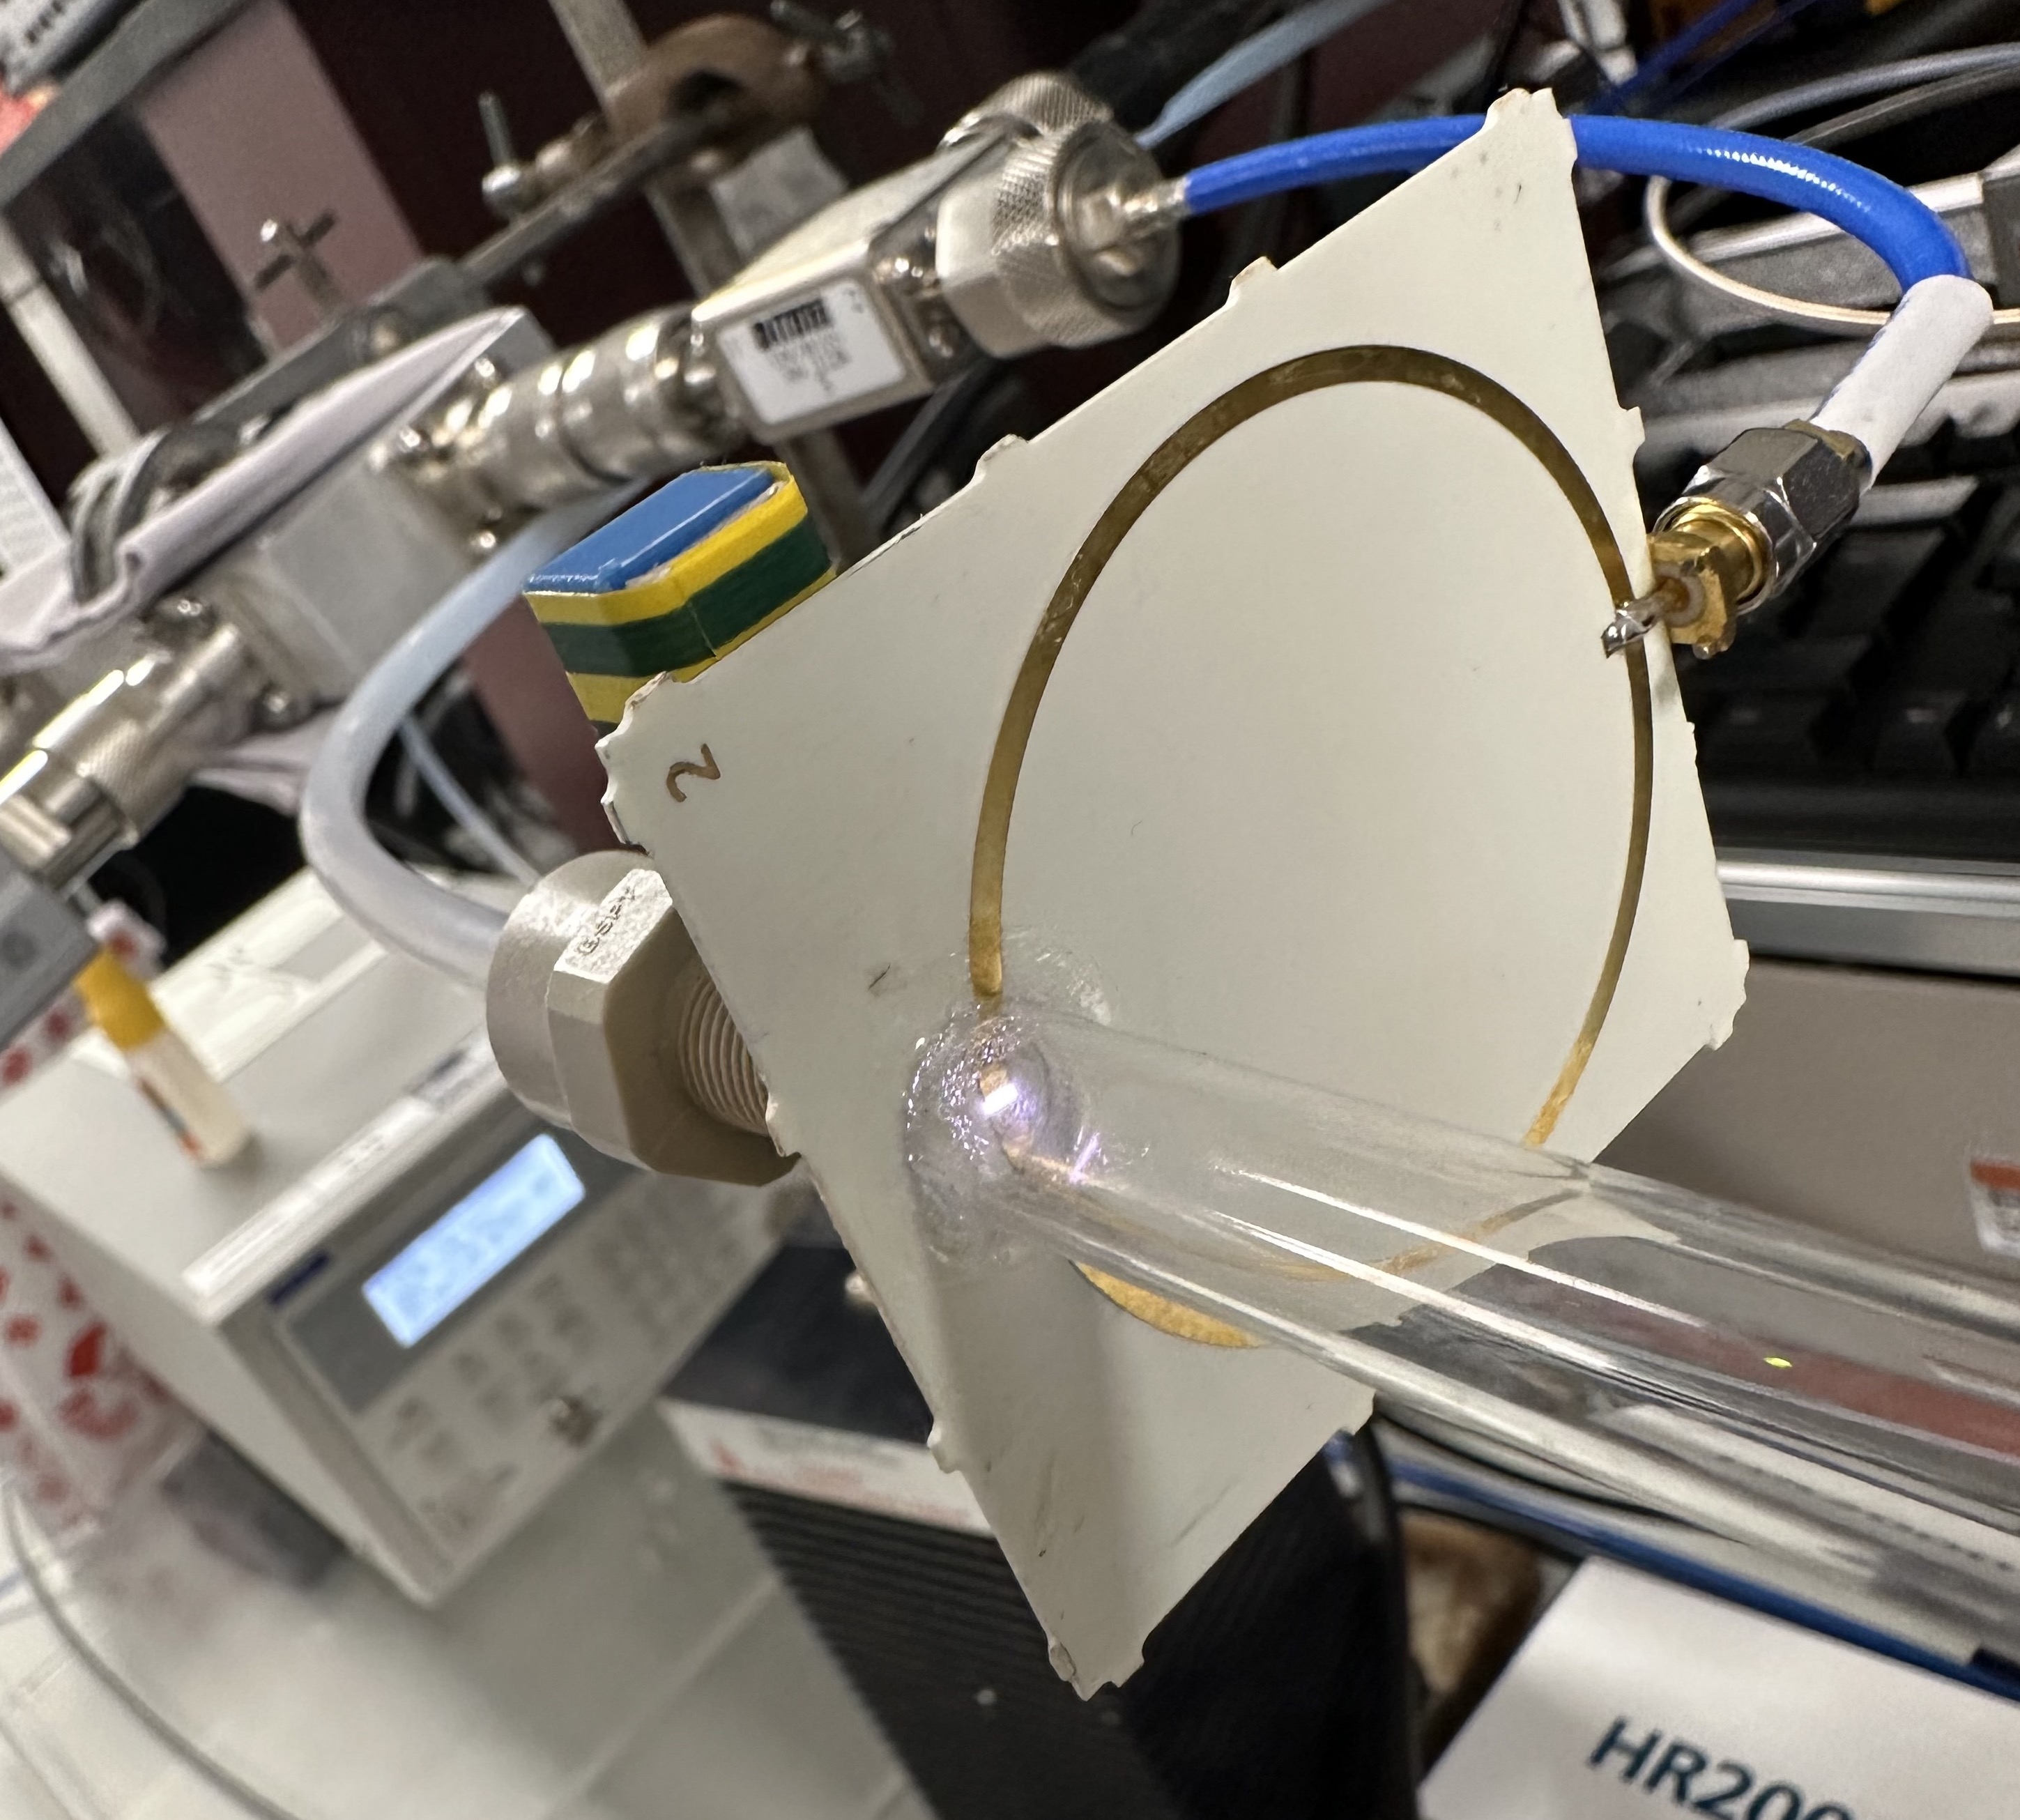
\includegraphics[width=0.55\linewidth]{chapter_4/figures/plasma.jpeg}
	\caption{Photograph of plasma discharge in the gap of the SRR.}
	\label{fig:SRR_plasma}
\end{figure}


In terms of the electronics, the the SRR is powered by a signal generator (Aim-TTi TGR2050), capable of generating frequencies up to 2 GHz, and a linear amplifier (Amplifier Research 50W1000A), with a maximum power output of 50 W. This is connected to a bi-directional coupler (Mini-Circuits ZGBDC20-33H-S+) to allow for the accurate measurement of the forward path and the reverse path of the microwave signals from the power supply and SRR respectively. These signals are monitored using a pair of USB power meters (Mini-Circuits PWR-SEN-4GHz, Mini-Circuits PWR-SEN-6LRMS-RC). One note regarding the power meters, the first power meter (PM$_1$) has a maximum power input of 100 mW, whilst the second one (PM$_2$) has a maximum reading of 10 mW. This is because, when the SRR is at resonance, only a small amount of signal is reflected back. 

\subsection{Device Performance}

%Now that the SRR was connected to the setup, there may be a slight change in the resonant frequency due to coupling with the rest of the electronics. However, with the use of the bi-directional couplers and the power meters, it is possible to find the frequency of resonance of the overall setup. This is achieved by keeping the input power of the power supply fixed, but varying its frequency. This way, the reading of the forward wave would be constant, with the power of the reflected wave changing. 
%
%For this, the input power was kept at a constant 10 mW. This was chosen as it was a low enough power to not ignite a plasma (which in turn would change the resonance characteristics of the SRR). As for the frequencies, a sweep was performed between 500 MHz to 600 MHz. The results of this can be seen in figure \ref{fig:reflected_power_SRR.png}. 
%
%\begin{figure}[h!]
%	\centering
%	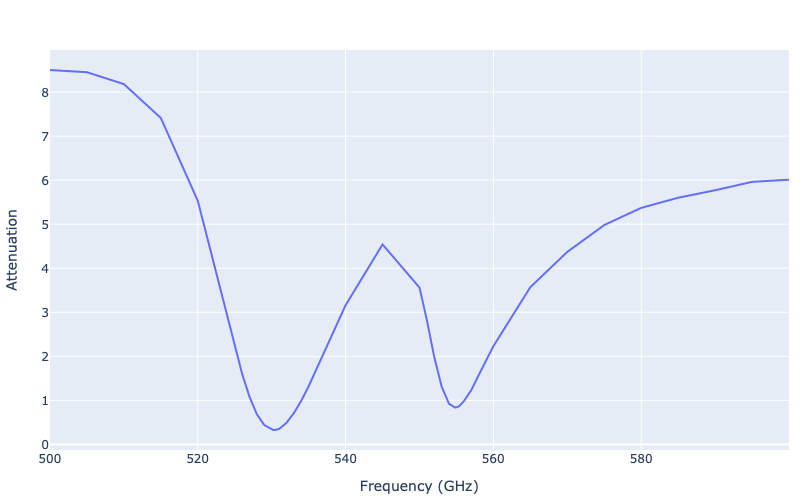
\includegraphics[width=\linewidth]{chapter_4/figures/reflected_power_SRR.png}
%	\caption{Reflection power of SRR when connected to the setup in mW.}
%	\label{fig:reflected_power_SRR.png}
%\end{figure}
%
%Two dips can be seen in the data. These dips correspond to the frequencies that cause an attenuation in the SRR. As expected, a drop in return power can be seen at 554 MHz (more precisely, it is 554.8 MHz), which is inline with the S-parameters measurements. However, a second dip is seen at 530 MHz (530.4 MHz specifically). Notably, this drop of return power at 530 MHz is lower than that of the drop at 554 MHz; with the readings being 0.33 mW and 0.84 mW respectively. As such, it can be concluded that 530.4 MHz is resonant frequency of the SRR connected to the rest of the setup. This conclusion is backed up by the fact that the plasma only ignites at that frequency, and not at 554 MHz.

Once ignition was achieved, the next steps were to evaluate the performance of the device. This was determined by evaluating was the ignition power of the SRR. This is because, igniting plasma at higher pressures tends to be slightly more inefficient compared to lower pressures. Thus, the ignition power was tested at various pressures to determine the minimum power required to get a plasma to from with the SRR. 

To obtain this data, first the pressure of the chamber was fixed. Then input power to the SRR was increased gradually until the self-ignition of the plasma. The power value was noted, and the input power was reduced back to the minimum value and the process was repeated. In total, there were five power readings taken at each pressure to account for outliers. This data is shown in figure \ref{fig:ignition_power}. Each point in the figure denotes the average ignition power at that pressure, with the error bars denoting the standard deviation in the data collected. Do note that x-axis of this graph was plotted in logarithmic scale. 

\begin{figure}[h!]
	\centering
	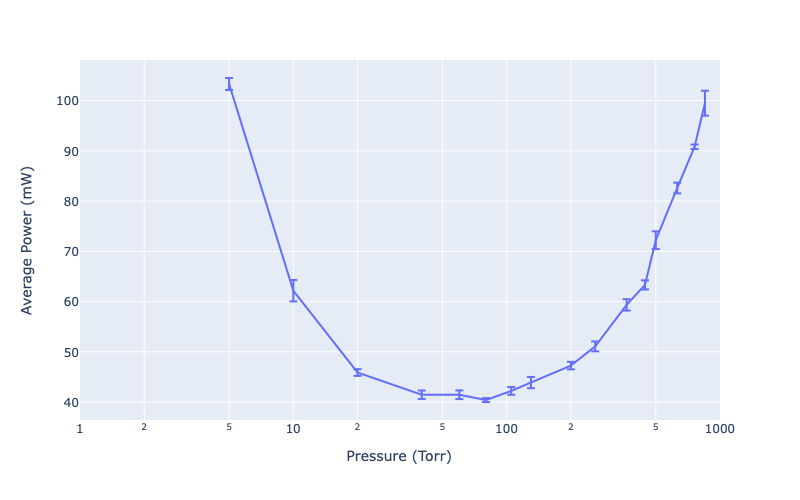
\includegraphics[width=\linewidth]{chapter_4/figures/ignition_power.png}
	\caption{Ignition power of SSR, in W, across a pressure range of 5 Torr to 850 Torr.}
	\label{fig:ignition_power}
\end{figure}

As seen by the graph, the minimum power required to ignite the plasma was just 4.04 W. While this is fairly small, it could be better as the real world quality factor of the SRR was lower than anticipated. While this minimum ignition power was achieved at 80 Torr, the power remained relatively low across a broad range of pressures, ranging from 40 Torr to 105 Torr, with the ignition power hovering around 4.1-4.2 W. As the pressure decreased below 40 Torr, the ignition power required increased steeply up to a pressure of 5 Torr where the readings maxed out the range of the power meter. It is also important to note that at 5 Torr, while the plasma self-ignited, it did take significantly longer when compared to the ignition at other pressures. As for pressures above 105 Torr, the ignition power also increased, though at a much slower rate. At 760 Torr, the average power required to ignite the plasma was 9.08 W. The testing was carried out past 760 to determine the upper bound pressure that a plasma could be ignited with the equipment in the setup; this value was at 850 Torr. 

From the data in figure \ref{fig:ignition_power}, it can be concluded that the most efficient way to ignite a plasma with this SRR would be to first pressurise the chamber to approximately 100 Torr. Then, once the plasma is ignited, the pressure can be increased back to 760 Torr. 

\pagebreak

\subsection{Pressure Drop across Orifice}

Another test done was to evaluate the pressure difference between both sides of the SRR. Since the size of the drill hole through the gap of the SRR was quite small, this would restrict the gas flow. This meant that as gas flowed through the orifice, it would accelerate and reach its maximum velocity just after the orifice. This point of maximum velocity is referred to as the \textit{vena contracta}. From Bernoulli's principle, it is known that an increase in a fluid velocity results in a drop in pressure. As the goal of this research to use  a co-reactant (trans-Stilbene) at atmospheric pressure in the carbon conversion process, the significance of this pressure drop needed to be known. An illustration of this pressure drop can be seen in figure \ref{fig:orifice_vena_contracta}. Note that while the pressure drop is at its greatest at the vena contracta, but there is also a net pressure drop well after the orifice.

\begin{figure}[h!]
	\centering
	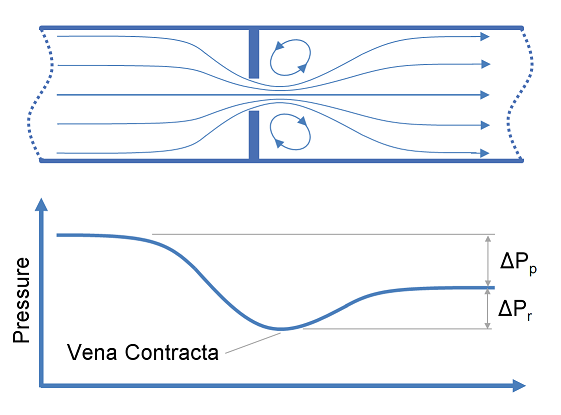
\includegraphics[width=0.75\linewidth]{chapter_4/figures/orifice-vena-contracta.png}
	\caption{Pressure drop across an orifice visualised. \cite{Neutrium}}
	\label{fig:orifice_vena_contracta}
\end{figure}

This drop in pressure can be determined analytically by using Bernoulli's equation as shown in equation \ref{eq:bernoulli_equation}. The derivation shown here would be for the case where orifice placed in horizontal pipework, as this is the orientation used in the setup shown in figure \ref{fig:SRR_setup}. Though the orientation of the pipework (and thus the orifice) for the final experiment with the co-reactant will be vertical, the impact of this change is minor as shown later in this subsection.

\begin{equation}
    P_1 + \frac{1}{2} \rho v^2_1 + \rho g h_1 = P_2 + \frac{1}{2} \rho v^2_2 + \rho g h_2
    \label{eq:bernoulli_equation}
\end{equation}

where $\rho$ is the density of the gas, $g$ is the acceleration due to gravity, $P$ is the pressure, $v$ is the gas velocity, and $h$ is the height of the gas. The subscripts denote the positions of the pressure, velocity, and height at different points in the pipework. In this case, point 1 denotes a location just before the orifice and point 2 is just after the orifice of the SRR.

For the case of horizontal flow, it can be assumed that there is a negligible change in elevation. The resulting equation when $h_1 = h_2$ is:
\begin{equation}
    P_1 + \frac{1}{2} \rho v^2_1  = P_2 + \frac{1}{2} \rho v^2_2
    \label{eq:bernoulli_equation_horizontal_case}
\end{equation}

Assuming that the velocity profiles at points 1 and 2 are uniform, the continuity equation can be shown to be:
\begin{equation}
    Q = A_1 v_1  = A_2 v_2 
    \label{eq:continuity_equation}
\end{equation}
where $Q$ is the flow rate and $A$ denotes the area of flow at the given points. 

Substituting the velocity terms in equation \ref{eq:bernoulli_equation_horizontal_case} with equation \ref{eq:continuity_equation}, and rearranging the pressure terms to the same side of the equation results in the expression:
\begin{equation}
    \Delta P = P_1 - P_2 = \frac{1}{2} \rho \left (\frac{Q}{A_2} \right )^2 - \frac{1}{2} \rho \left (\frac{Q}{A_1} \right )^2
    \label{eq:bernoulli_equation_horizontal_case_with_continuity}
\end{equation}


Since the tubing used and the orifice or the SRR are concentric, the areas $A_1$ and $A_2$ are simply $\frac{\pi}{4} d_1^2$ and $\frac{\pi}{4} d_2^2$ respectively. Because $d_2 < d_1$, a new parameter can be introduced to describe the relationship between the size of the orifice and the tubing. This parameter, called $\beta$, is defined as:
\begin{equation}
    \beta = \frac{d_2}{d_1}
\end{equation}

\newpage
This term can be added to \ref{eq:bernoulli_equation_horizontal_case_with_continuity} as follows:

\begin{equation}
\begin{aligned} 
\Delta P &= \frac{1}{2} \rho \left (\frac{Q}{A_2} \right )^2 - \frac{1}{2} \rho \left (\frac{q}{A_1} \frac{A_2}{A_2} \right )^2 \\ 
\Delta P &= \frac{1}{2} \rho \left (\frac{Q}{A_2} \right )^2  \left [1 - \left( \frac{A_2}{A_1} \right )^2 \right ] \\
\Delta P &= \frac{1}{2} \rho \left (\frac{Q}{A_2} \right )^2  \left [1 - \left( \frac{d_2^2}{d_1^2} \right )^2 \right ] \\
\Delta P &= \frac{1}{2} \rho \left (1 - \beta^4 \right )  \left (\frac{Q}{A_2} \right )^2 
\end{aligned}
\label{eq:ideal_pressure_drop_equation}
\end{equation}

The expression above is the \textit{ideal} equation for pressure difference through an orifice in horizontal pipework. However, in practice the flow rate through the orifice will be smaller than the expected flow rate due to the geometry of the hole itself. This can be rectified by adding a discharge coefficient term to the final line of equation \ref{eq:ideal_pressure_drop_equation}. The discharge coefficient, $C_d$ is the ratio of actual discharge compared to the ideal discharge at the end of the orifice. An intuitive explanation of this the ratio between the area of flow at the vena contracta compared to the area of the orifice. 

Adding this discharge coefficient term results in the final equation:

 \begin{equation}
    \Delta P = \frac{1}{2} \rho \left (1 - \beta^4 \right )  \left (\frac{Q}{C_d A_2} \right )^2
    \label{eq:better_ideal_pressure_drop_equation}
\end{equation}

Note that in the equation above, the only independent variable is the flow rate. Thus, it can be said that $\Delta P \propto Q^2$. 

To test this relationship, the setup in figure \ref{fig:SRR_setup} was modified by adding a second pressure sensor. An illustration of this setup can be seen in figure \ref{fig:pressure_drop_test}, where PS$_1$ is the original pressure sensor at the main chamber and PS$_2$ corresponds to the new pressure sensor. The gas from the mass flow controller is fed through a pressure sensor located before the SRR orifice. The pressure after the orifice was measured from the pressure sensor located in the chamber. These are not the ideal locations to measure the pressure, but should be sufficient to determine the significance of any pressure drop.

\begin{figure}[h!]
	\centering
	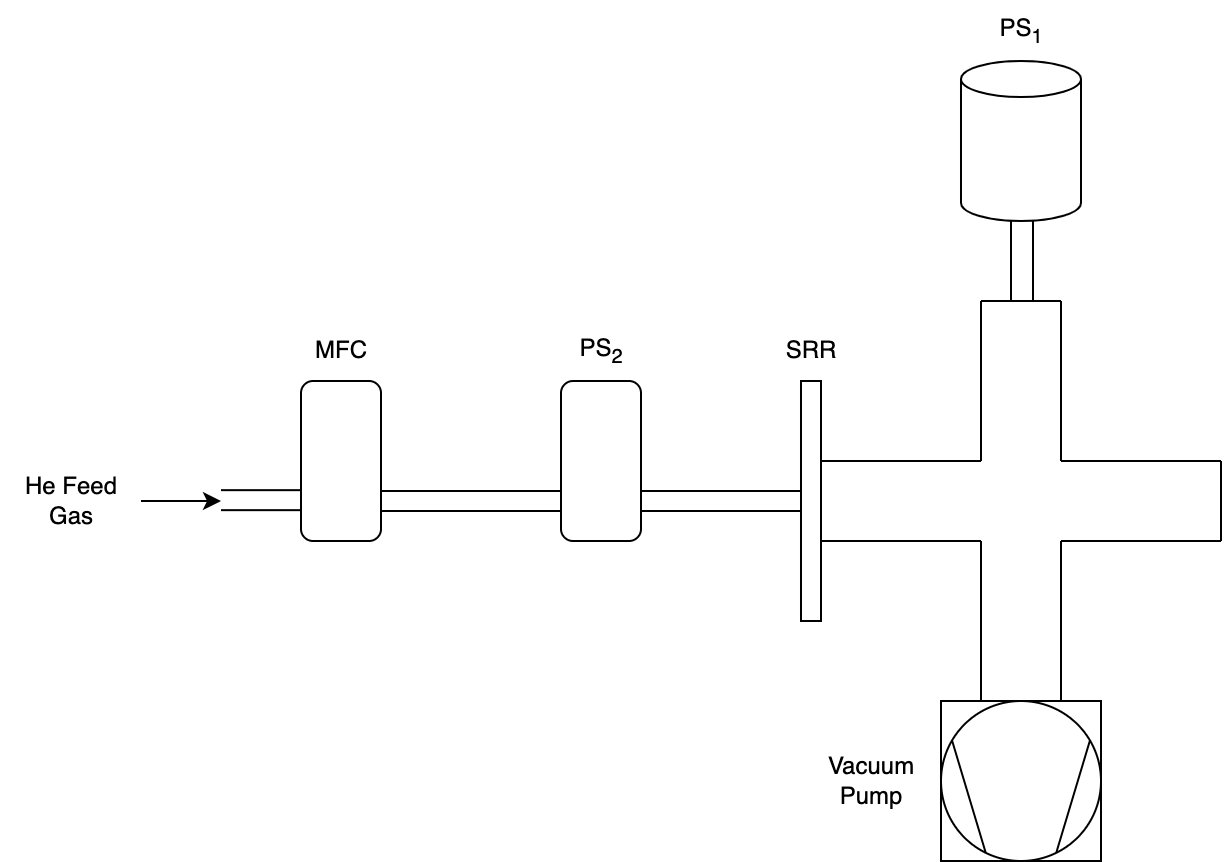
\includegraphics[width=0.7\linewidth]{chapter_4/figures/pressure_drop_test.png}
	\caption{Schematic of setup used to determine the pressure drop through orifice.}
	\label{fig:pressure_drop_test}
\end{figure}

Both the SRR with a single hole and multiple holes were tested. The mass flow controller used had a range of up to 200 sccm, which determined the maximum flow rate possible. As for the minimum flow rate, values under 20 sccm would cause the valve of the mass flow controller to oscillate open and closed which meant that the flow rate was no longer uniformed. The results of this test can be seen in table \ref{tb:pressure_drop_results}.

\begin{table}[h!]
\centering
\caption{Comparison of pressure drop across single-hole and multi-hole SRR orifices across different flow rates.}
\begin{tabular}{rll}
Q (sccm) & $\Delta$P - Single hole (Torr) & $\Delta$P - Multi hole (Torr) \\
\hline
30               & 0.716 $\pm$ 0.050     & 0.348 $\pm$ 0.086    \\
50               & 1.341 $\pm$ 0.050     & 0.504 $\pm$ 0.076    \\
70               & 3.415 $\pm$ 0.124     & 0.601 $\pm$ 0.076    \\
100              & 5.052 $\pm$ 0.068     & 0.928 $\pm$ 0.081    \\
120              & 6.318 $\pm$ 0.063     & 1.210 $\pm$ 0.071    \\
150              & 8.582 $\pm$ 0.061     & 1.615 $\pm$ 0.072    \\
180              & 10.877 $\pm$ 0.088    & 2.000 $\pm$ 0.069    \\
200              & 12.598 $\pm$ 0.063    & 2.275 $\pm$ 0.102   
\end{tabular}
\label{tb:pressure_drop_results}
\end{table}


Based on equation \ref{eq:better_ideal_pressure_drop_equation}, it is possible compare the theoretical results to the ones measured. However, this is only applicable to the SRR with a single hole as the equation is only valid for simple concentric geometries. The fixed parameters used to model the pressure drop are seen in table \ref{tb:params_for_pressure_drop_results}. A discharge coefficient of $C_d = 0.6$ which selected as it was a typical values used to model sharp edged orifices \cite{EdgarONTO, Woodward2014}. 

\begin{table}[h!]
\centering
\caption{Parameters used in equation \ref{eq:better_ideal_pressure_drop_equation}.}
\begin{tabular}{crl}
Parameters & Values & Units \\
\hline
$\rho$     & 0.167  & g L$^{-1}$ \\
d$_1$      & 4      & mm         \\
d$_2$      & 0.24   & mm         \\
$\beta$    & 0.06   &            \\
A$_2$      & 0.0452 & mm$^2$     \\
C$_d$      & 0.6    &      
\end{tabular}
\label{tb:params_for_pressure_drop_results}
\end{table}

A graph of the the comparison between theoretical and measured pressure drops can be seen in figure \ref{fig:pressure_difference}. It can be seen that the measured results are within the same order of magnitude to the theoretical values. However, there are sizeable discrepancies between those numbers. 

\begin{figure}[h!]
	\centering
	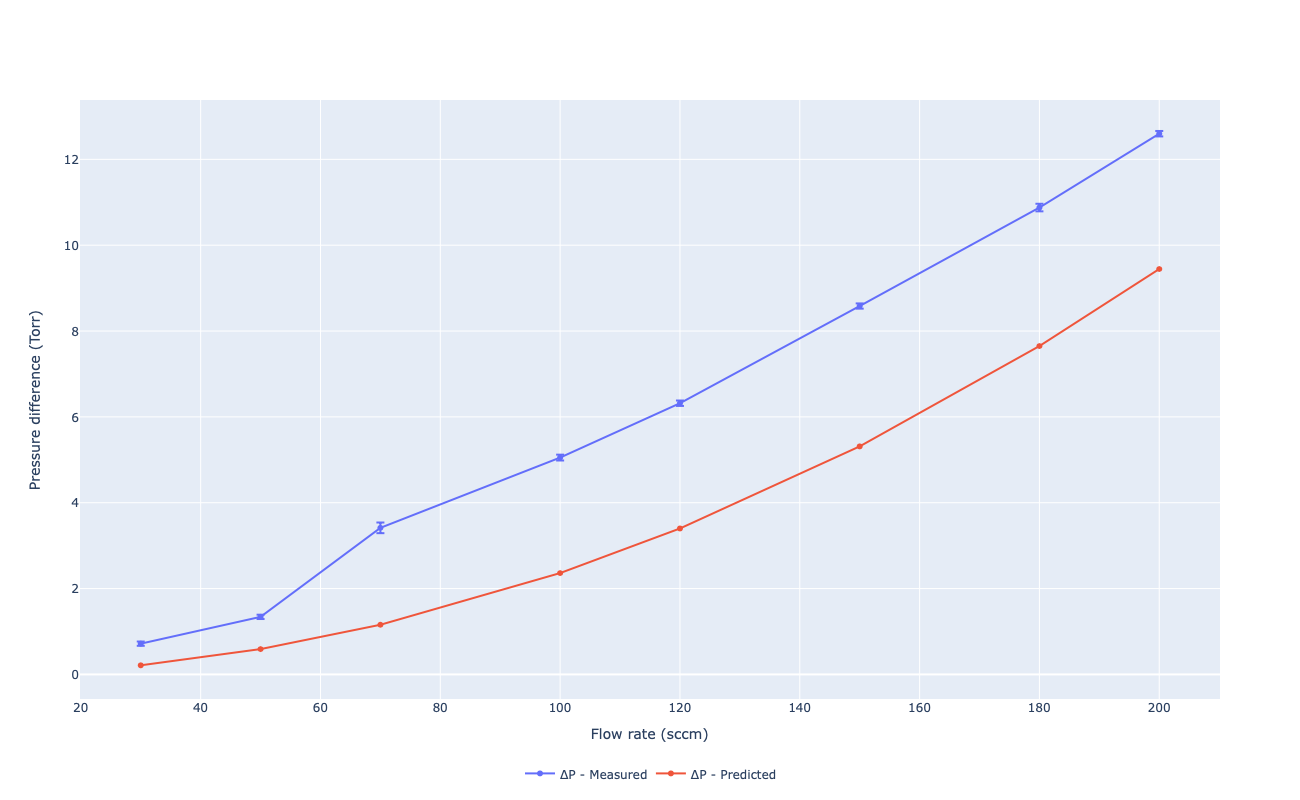
\includegraphics[width=\linewidth]{chapter_4/figures/pressure_difference.png}
	\caption{Comparison of true and predicted results for pressure drop across SRR with single hole orifice.}
	\label{fig:pressure_difference}
\end{figure}

The are numerous possible reasons for this, with the largest being that the model in equation \ref{eq:better_ideal_pressure_drop_equation} is incomplete. Adding factors such as the expansion coefficient (to take account the difference between compressible and incompressible flows) and the specific heat ratio (which describes the relationship of the heat capacity of the gas at constant volumes and pressures) could improve model, though the values for these terms need to be determined experimentally. Another possible reason is that the assumed value of C$_d$ is simply incorrect. Finally, as stated previously, the location of the pressure sensors are simply too far from the SRR, thus the readings at the measured locations not correspond to that in equation \ref{eq:better_ideal_pressure_drop_equation}. Nonetheless, the model is a sufficient  approximation for the purposes of this project.

Another point to note on equation \ref{eq:better_ideal_pressure_drop_equation} was that it was derived for a setup with horizontal pipework. For the case with a vertical gas flow, the change in elevation needs to be taken into account. Modifying the equation to include these terms results in:
\begin{equation}
    \Delta P = \frac{1}{2} \rho \left (1 - \beta^4 \right )  \left (\frac{Q}{C_d A_2} \right )^2 - \rho g \Delta h
    \label{eq:better_ideal_pressure_drop_equation_for_vertical}
\end{equation}
where $\Delta h$ is the height difference between the two points. 

However, as the thickness of the SRR is not particularly large and that the device will be located relatively close to the surface of the liquid co-reactant, the impact of the added height term is negligible. To give an example, a 10 mm drop in height would cause the pressure to drop by only 0.0001 Torr. As such, the measured results indicate that the pressure drop across the SRR is not significant, thus should not cause issues when operating with the co-reactant.

\pagebreak


\section{Flow of gases}
\subsection{Helium only}

%\subsection{Flow Rate and Input Power}

The only variable that could not simulated with XOOPIC, aside for the geometry of number of orifices on the SRR, was the flow rate through the device. As such, the flow rate through the SRR were tested with the Helium feed gas on both designs.

To evaluate the the impact on changing the flow rate, the light intensity of the plasma was used as a proxy for its temperature. The higher the light intensity of the plasma, the more energetic it is, thus the more likely ionising collisions are occurring. The light intensities were determined via optical emission spectroscopy, with the spectrometer located opposite the SRR as shown in figure \ref{fig:he_testing_setup}.

\begin{figure}[h!]
	\centering
	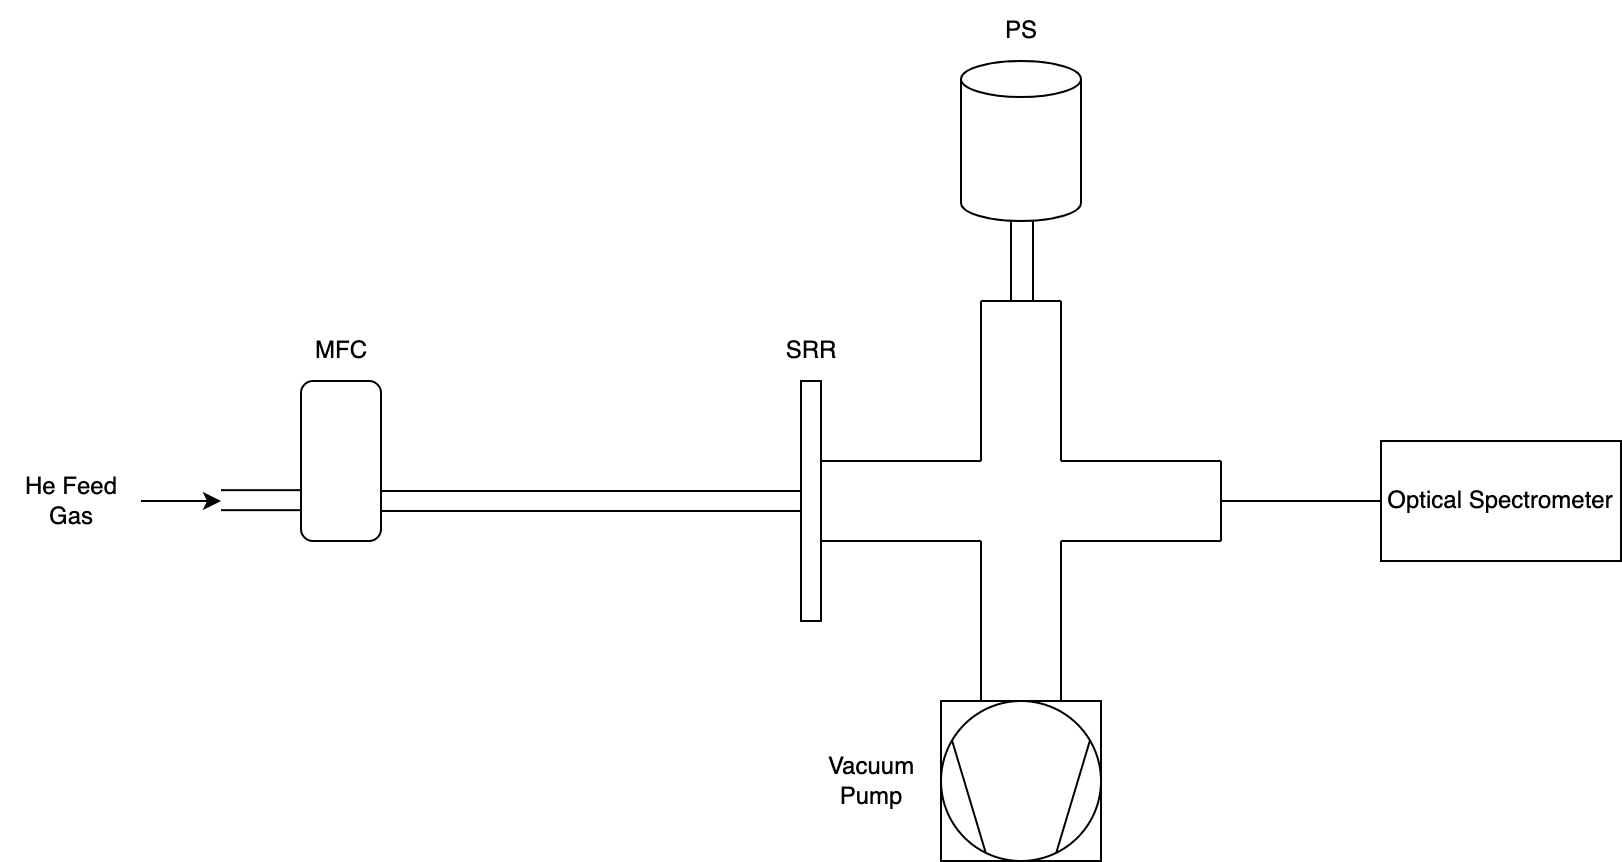
\includegraphics[width=0.8\linewidth]{chapter_4/figures/he_testing_setup.png}
	\caption{Schematic of setup used for He feed gas to ignite SRR.}
	\label{fig:he_testing_setup}
\end{figure}


The spectrometer used was the \textit{Ocean Optics USB2000+ Spectrometer}. These spectrometers work by focusing the light received onto a grating, which spreads the light out into a spectrum. Once spread out, the light is focused onto a detector which is then interpreted by the Ocean Optics software. An illustration of the light path through the spectrometer can be seen in figure \ref{fig:optical_spectrometer} from the spectrometer datasheet. 

\begin{figure}[h!]
	\centering
	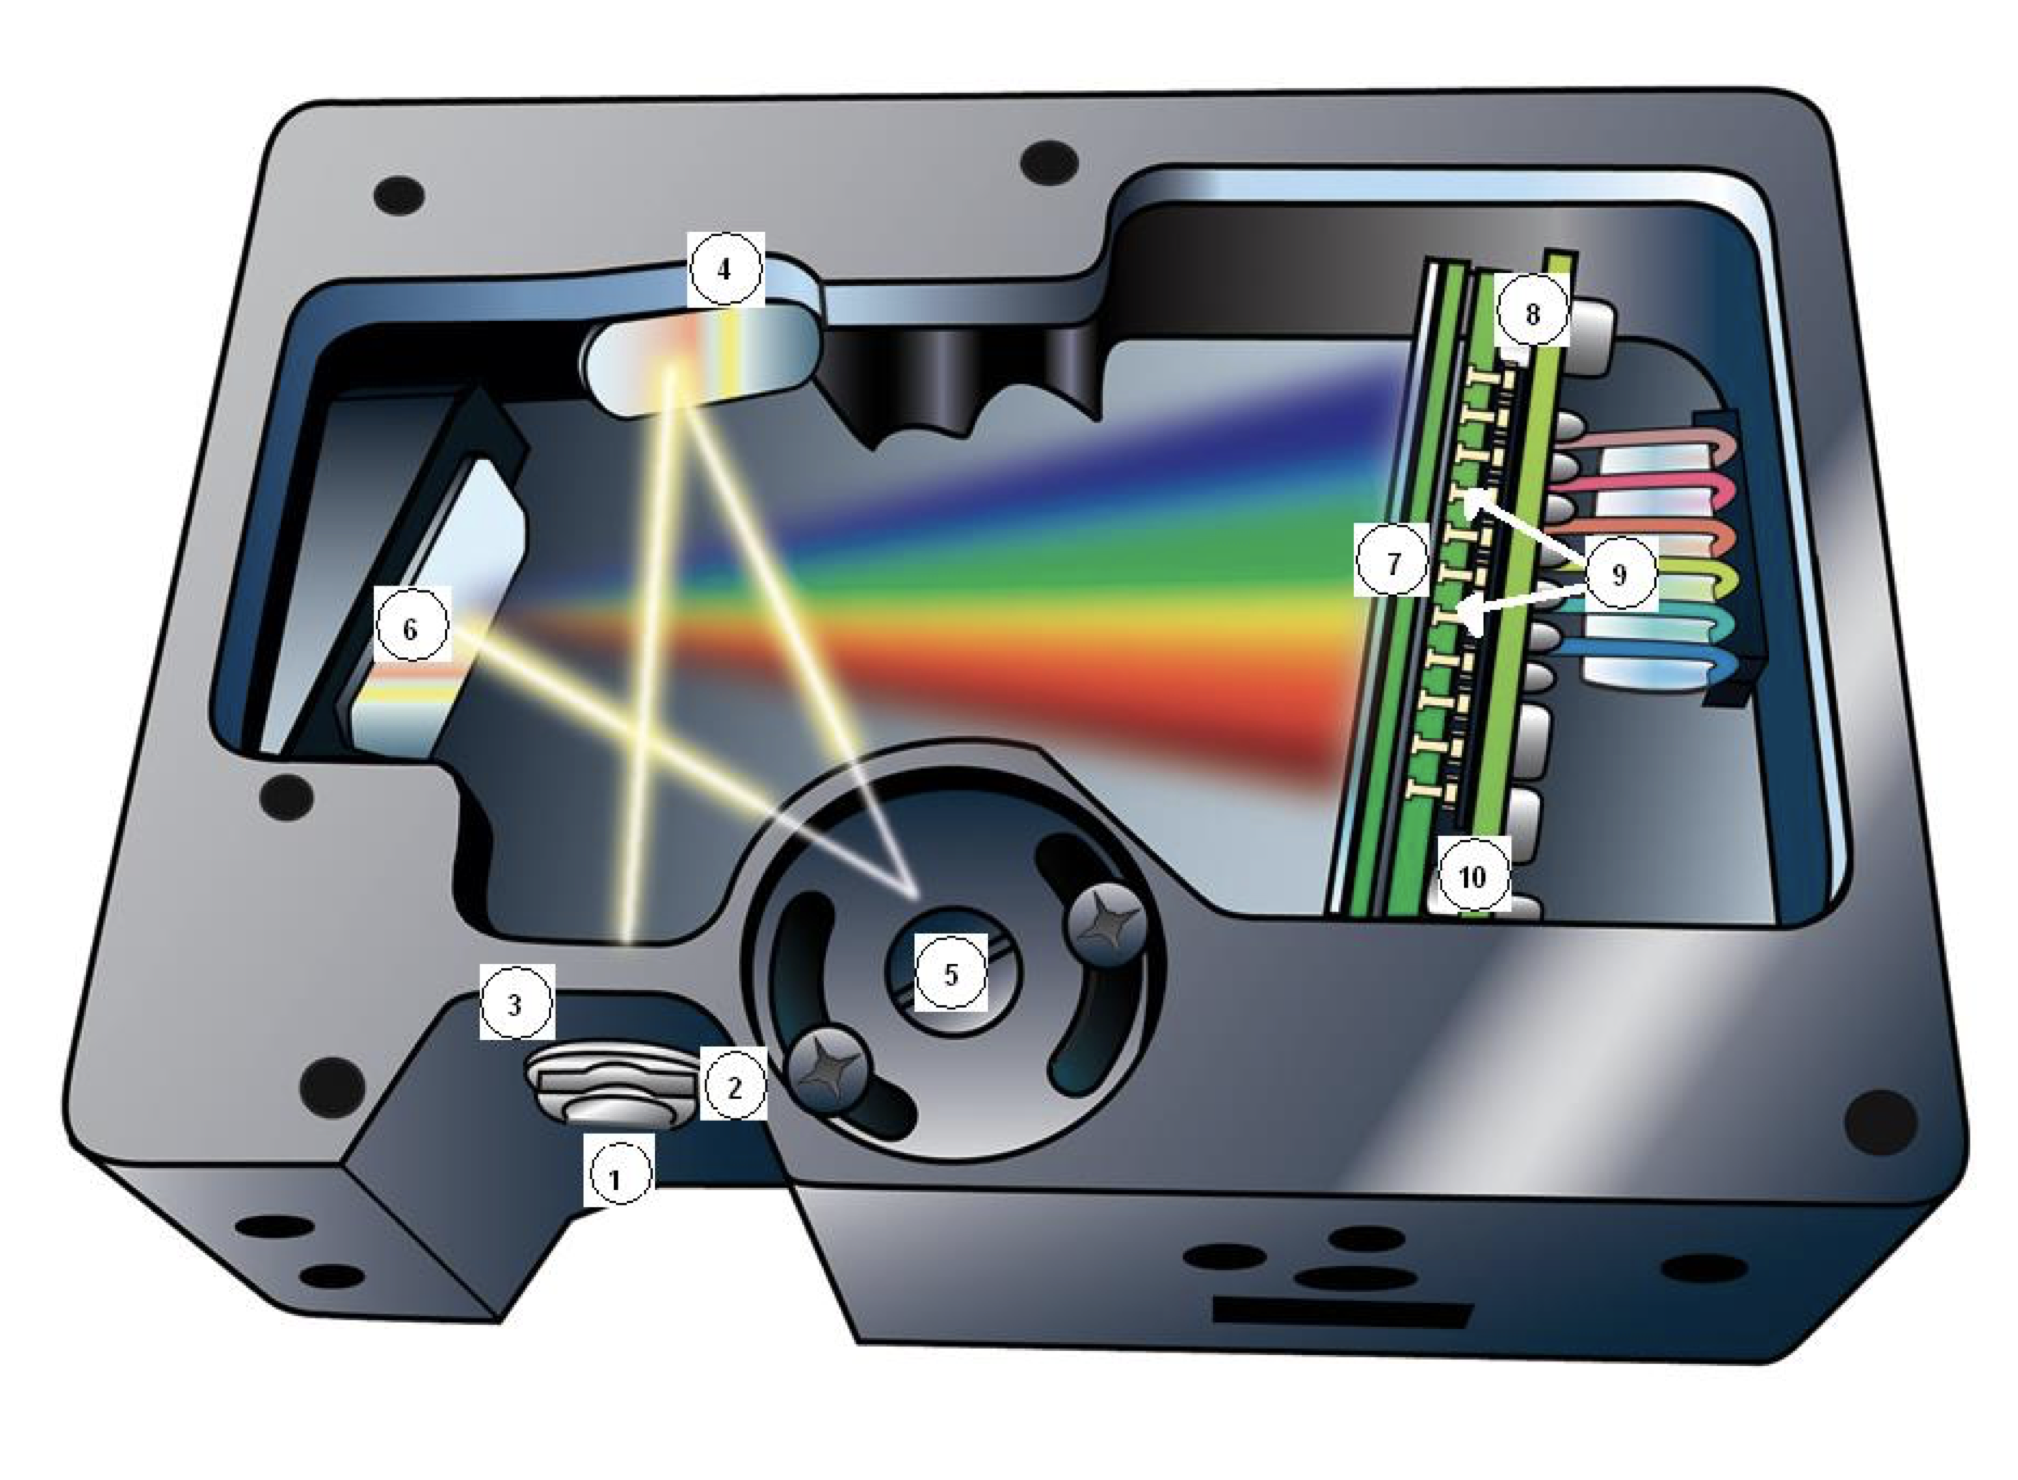
\includegraphics[width=0.6\linewidth]{chapter_4/figures/optical_spectrometer.png}
	\caption{Schematic for Ocean Optics spectrometer \cite{oo_spectrometer}.}
	\label{fig:optical_spectrometer}
\end{figure}

The spectrometer used has a range between 200 to 900 nm, with an optical resolution of roughly 0.5 nm. However, the viewport opposite the SRR used borosilicate glass, which blocks the transmission of light below 300 nm. However, this is not an issue since the wavelengths of light of interest closer to the red part of the spectrum. The emission peaks for Helium are located at 587.5, 667.8, 706.5, and 728.1 nm. The peaks for a control test (where $Q = 50$ sccm and $P = 5$ W) are shown in figure \ref{fig:he_optical_spectra}. The other peaks observed were mainly N$_2$ impurities in the gas, which are present since they have a much lower ionising potential (approximately 15.6 eV) than that of He (25.6 eV). Additionally, an atomic O peak was present at 777 nm. 

To evaluate the impact of flow rate on the light intensity of the plasma, the strong He peak (which was at 587 nm) was taken. Its intensity was measured at flow rates between 20-50 sccm, across both orifice designs. These results are shown in table \ref{tb:light_intensity_flow_rate_he}.

\begin{table}[h!]
\centering
\caption{The effect of flow rate on the light intensity of the He plasma.}
\begin{tabular}{rll}
Q (sccm) & Intensity (a.u) - Single hole & Intensity (a.u) - Multi hole \\
\hline
20       & 3724                          & 4884                         \\
30       & 4222                          & 4810                         \\
40       & 4498                          & 4789                         \\
50       & 4427                          & 4798                        
\end{tabular}
\label{tb:light_intensity_flow_rate_he}
\end{table}

\begin{figure}[h!]
	\centering
	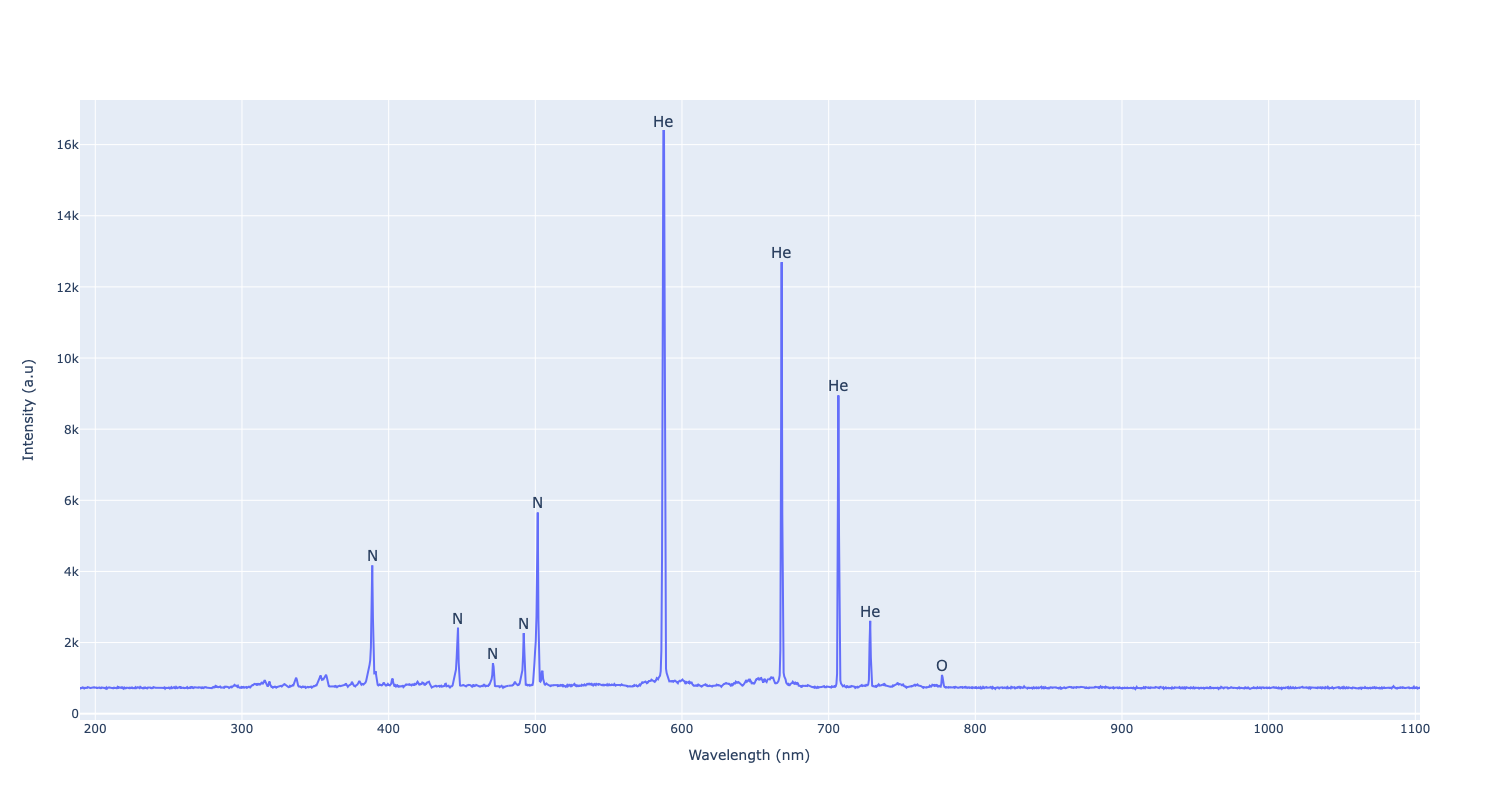
\includegraphics[width=\linewidth]{chapter_4/figures/he_optical_spectra.png}
	\caption{Optical emission spectra of He plasma with SRR.}
	\label{fig:he_optical_spectra}
\end{figure}



%
%Since the pressure of the plasma and distance between electrodes are fixed parameters governed by the intended experiment and geometry of the SRR device respectively, and the plasma only ignites within a narrow band of frequencies, this means that there are only two parameters that govern the characteristics of the plasma for the SRR. These are the flow rate through the hole(s) within the gap of the SRR and the power used to drive it. As such it would be useful to characterise these parameters to get a better understanding of the device, and to determine the ideal conditions for subsequent experiments. 



%However, this is not much of an issue since the wavelengths of light of interest lie primarily in the near infrared part of the spectrum. This is because this is where the emission peaks of Helium are located. The  peaks observed for a control test with a flow rate 50 sccm at a power of 5W is shown in figure \ref{}.
%
%To assess this, each parameter would be tested independently, and the dependant variable would be the light intensity of the plasma as a proxy for its temperature. The higher the light intensity of the plasma, the more energetic it is, thus the more likely ionising collisions are occurring. The light intensities were determined via optical spectroscopy, using the \textit{Ocean Optics USB2000+ Spectrometer}. The light entering the spectrometer hits a grating that separates the wavelengths of light onto a detector. This gives the detector a wavelength range between 200 to 900 nm, with an optical resolution of roughly x nm. However, due to the use of borosilicate glass for the viewport opposite the plasma, the transmission of light below roughly 300 nm drops to zero. However, this is not much of an issue since the wavelengths of light of interest lie primarily in the near infrared part of the spectrum. This is because this is where the emission peaks of Helium are located. The  peaks observed for a control test with a flow rate 50 sccm at a power of 5W is shown in figure \ref{}. In this test, the Helium peaks seen were at 667.8, 686.7, and, 706.5 nm. As such for the subsequent tests, only the light intensities at those values would be measured. 
%
%The first parameter to be tested would be the flow rate of feed gas through the SRR. A range of values were tested between 20 to 200 sccm of Helium. The maximum value was governed by the limit of the mass flow controller, while the minimum of 20 sccm was selected because values under that would cause the valve of the mass flow controller to oscillate open and closed, as such the flow rate would no longer be uniform. 

\subsection{Helium with Carbon Dioxide}
\label{subsec:helium_and_co2}

As seen in figure \ref{fig:co2_testing_setup}, CO$_2$ gas was introduced into the system with a second mass flow controller. Since both mass flow controllers were calibrated for their respective gases, this meant that that the CO$_2$ concentration of the gas mixture through the SRR is governed as the ratio of the CO$_2$ flow rate to the total flow rate. 

\begin{figure}[h!]
	\centering
	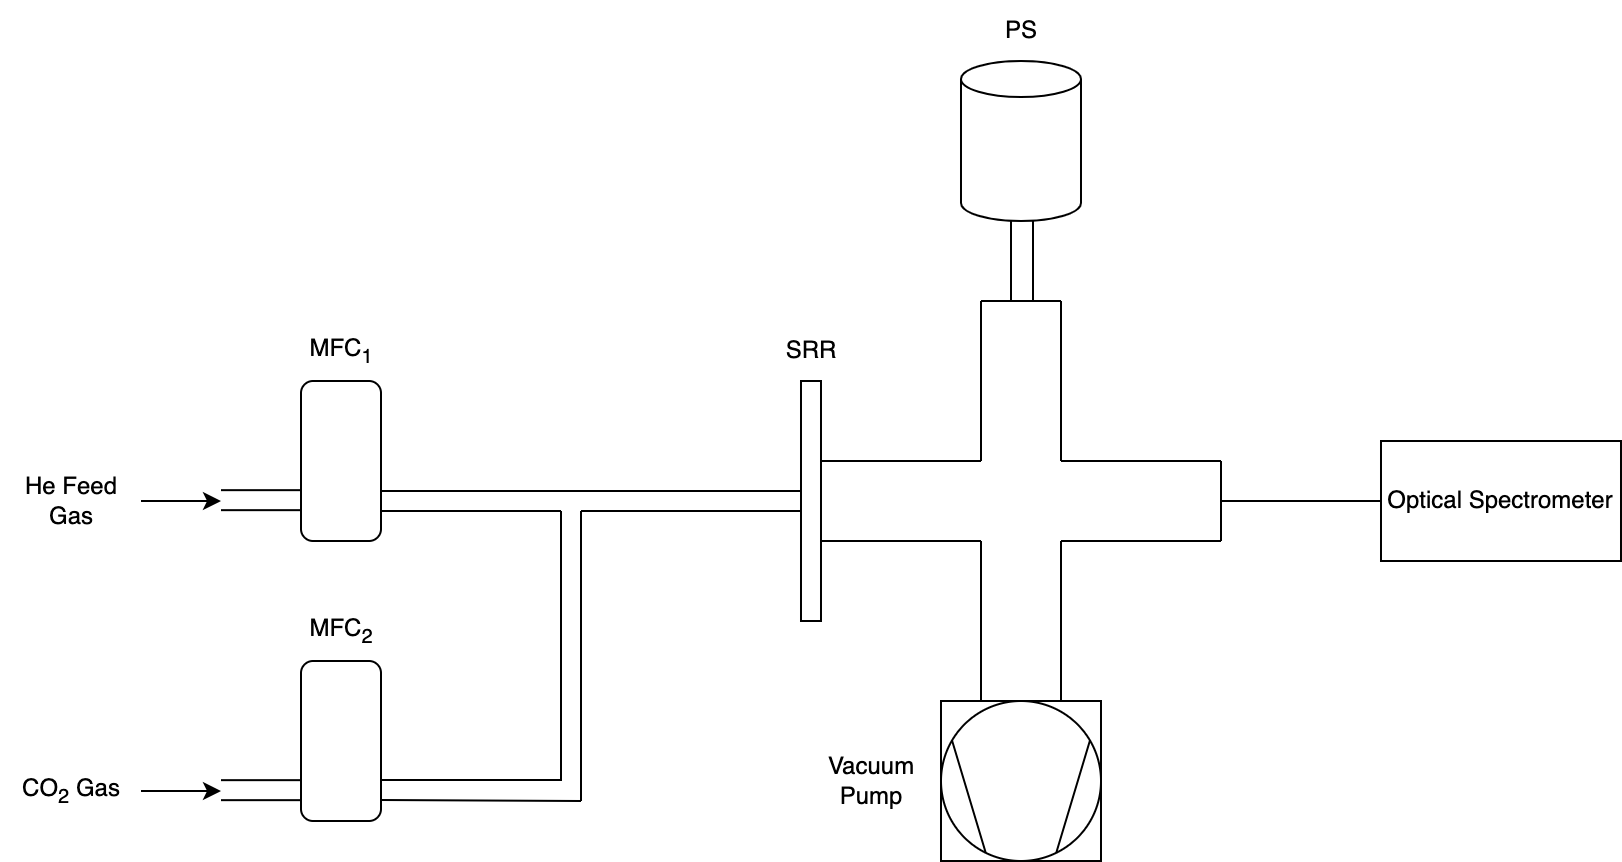
\includegraphics[width=0.8\linewidth]{chapter_4/figures/co2_testing_setup.png}
	\caption{Schematic of setup used for He-CO$_2$ gas mixture to ignite SRR.}
	\label{fig:co2_testing_setup}
\end{figure}

To visualise the impact of CO$_2$ concentration on the plasma, optical spectroscopy was used again. Keeping the total flow rate through the SRR constant at 50 sccm, the CO$_2$ concentration was increased from a $0\%$ to a $2.5\%$ gas mixture. These results can be seen in table \ref{}. 

It can be seen that as the concentration of CO$_2$ in the gas mixture increases, the intensity of the plasma drops. At a $2.5\%$ CO$_2$ concentration, the light intensity of the Helium peaks drop to zero as the plasma is extinguished. One thing to note that was not visible in the figure was that the plasma at $2\%$ CO$_2$ was quite unstable, in the sense that in some the tests the plasma would extinguish but not in others. As such when determining the ideal concentration of CO$_2$ to be used, a tradeoff between the amount of CO$_2$  available to react versus the plasma performance was required. In the end a $1\%$ CO$_2$ gas mixture was selected. 
%This value was inline with some other experiments involving Helium plasma jets at atmospheric pressure \cite{}. 

With the optical spectroscopy, the intention was also to detect the excitation peaks from the CO$_2$. This could be used later for the control system for regulating the concentration of CO$_2$ when recirculating the gases (seen in the next chapter). However, the CO$_2$ molecule itself does not have any excitation peaks in the optical spectrum. Instead, one has to rely on peaks from CO$_2^+$ and CO. For the former, these peaks are typically found at 337.0, 354.6, 362.1, and 396.1 nm \cite{Pearse1976}. However, the issue is that these peaks typically also very similar to nitrogen peaks. As for the CO peaks, these are typically referred to as the Ångström system and can be found at 451.1, 483.5, 519.8, 561.0, and 608.0 nm \cite{Pearse1976}. The full optical spectra for a $0\%$  and $1\%$ CO$_2$ concentration can be seen in figure \ref{fig:he_co2_optical_spectra}. In the figure, the intensity of the light (seen on the y-axis) has been normalised to the peaks of Helium. This was done to show the relative changes of the peaks as the flow rate of Helium is effectively constant.

\begin{figure}[h!]
	\centering
	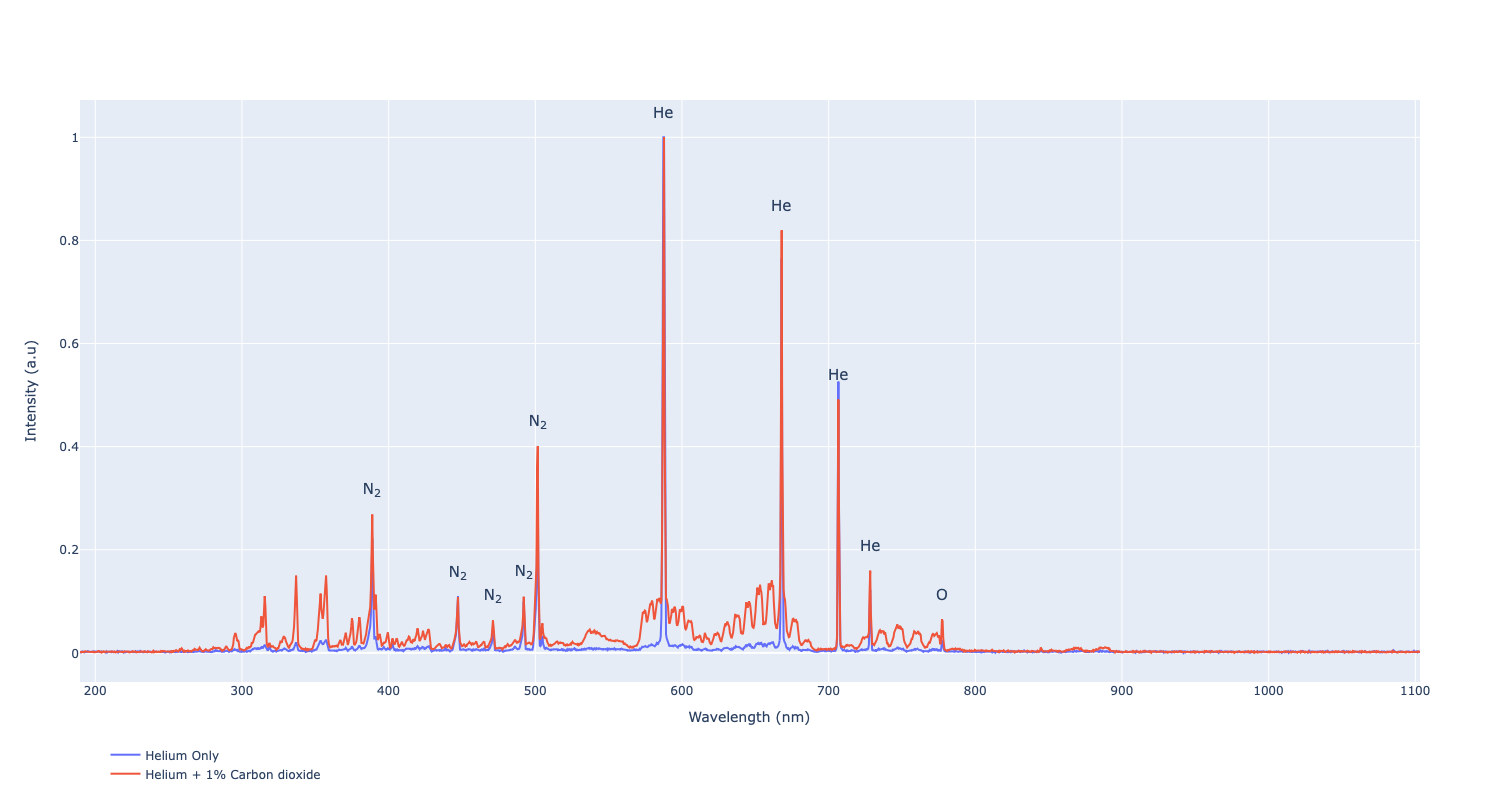
\includegraphics[width=\linewidth]{chapter_4/figures/he_co2_optical_spectra.png}
	\caption{Comparison of optical emission spectra of He only plasma and (1\%) CO$_2$-Helium plasma.}
	\label{fig:he_co2_optical_spectra}
\end{figure}

As seen from the figure, there are unfortunately no CO peaks. This could mean one of two possibilities. The first is that there is no CO$_2$ dissociations occurring in the plasma. However, due to the carbon deposits on the surface of SRR visible in figure \ref{fig:carbon_deposits_on_SRR}, this is very unlikely. The more likely reason is that there is not sufficient energy to excite the CO molecules in the optical spectra. This is further evident as it can be seen that there is an increase in atomic oxygen, which could only come from the dissociation of the CO$_2$ molecule. 

\begin{figure}[h!]
	\centering
	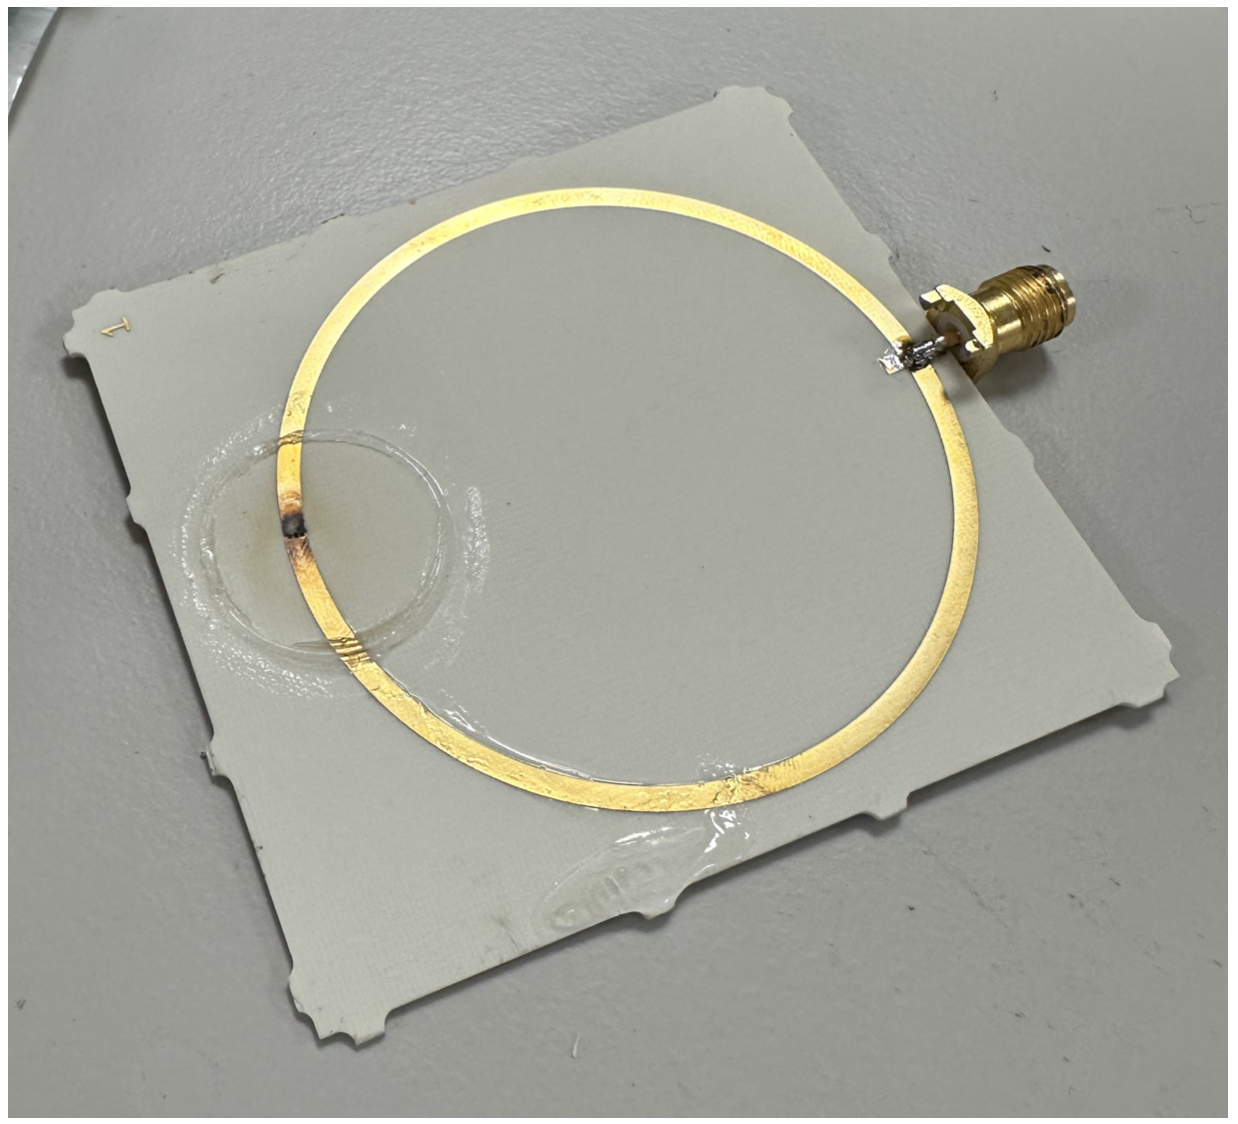
\includegraphics[width=0.75\linewidth]{chapter_4/figures/carbon_deposits_on_SRR.png}
	\caption{Photograph of carbon deposits on SRR.}
	\label{fig:carbon_deposits_on_SRR}
\end{figure}

\subsubsection{FTIR Analysis}

Because of this, an alternative test was required to ascertain the approximate CO$_2$ concentration in the system. This was achieved using Fourier-transform infrared spectroscopy (FTIR). The notable difference between the optical spectroscopy used above which measured the emission spectra of molecules and atoms, the FTIR detects the absorption spectra; which as the name suggests is the amount of light at a given frequency that is absorbed by the sample.

An illustration of how the FTIR works can be seen in figure \ref{fig:ftir_inteferometer}. In essence, it can be explained as follows. A beam of light that contain many frequencies of light is sent through the sample, and the detector measures the amount of light absorbed. Then the beam is changed to contain a different set of frequencies, and this process is repeated several times over a short period of time. These beams of light are referred to as interferograms. These interferograms are then decoded an algorithm called a  Fourier transform. To generate the beam of light going into the sample, a broadband light source is pointed to a beam splitter, which in turn is transmitted to a set of mirrors. By varying the distance of the moving mirror, constructive and destructive interference is observed in the recombined beam which results in the many frequencies.

\begin{figure}[h!]
	\centering
	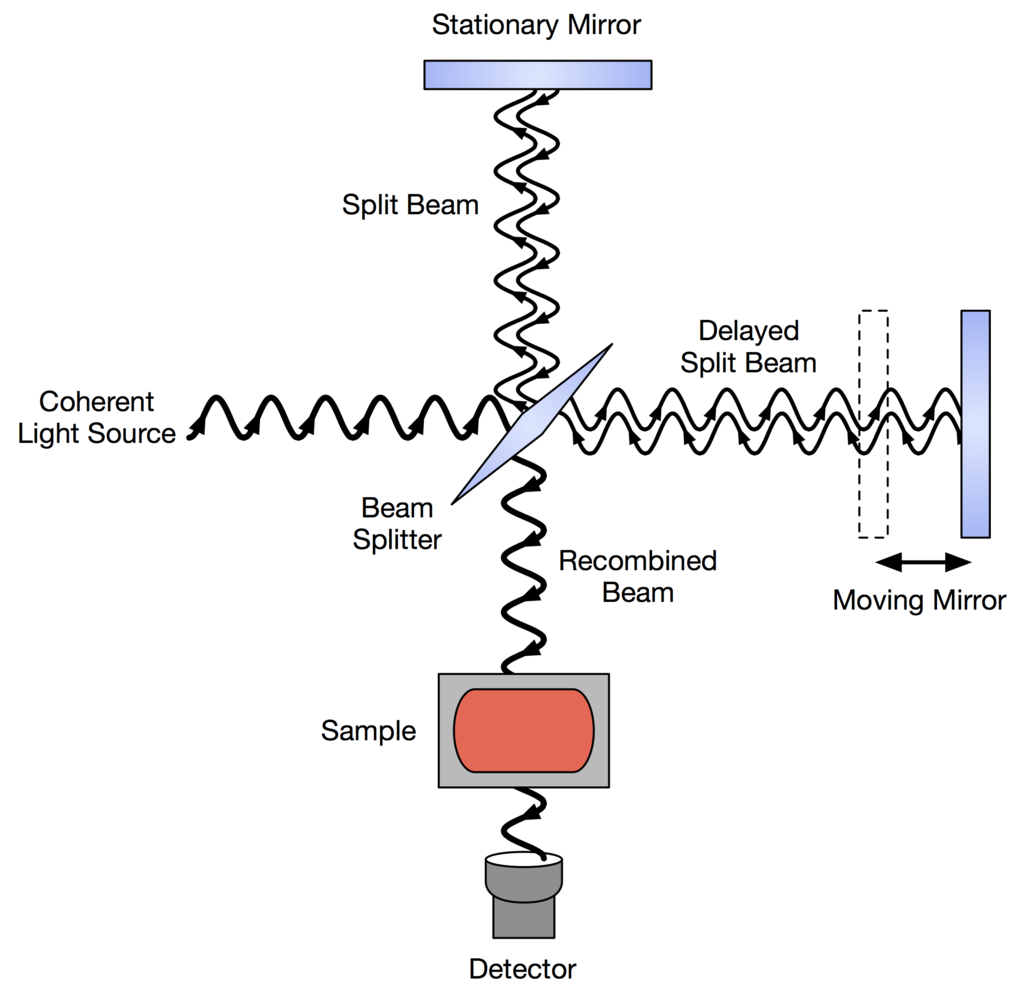
\includegraphics[width=0.6\linewidth]{chapter_4/figures/FTIR_Interferometer.png}
	\caption{Schematic of Fourier-transform infrared spectroscopy (FTIR) inteferometer.}
	\label{fig:ftir_inteferometer}
\end{figure}

To test the gas mixture, a \textit{Jasco FT/IR-4700} was used. The device was set up in-between the primary chamber of the SRR and the pump. In the infrared spectrum, CO$_2$ has a pair of strong absorption peaks at approximately 4255 nm. Typically when using IR spectroscopy, the measurement of wavenumber is used rather than the wavelength. The wavenumber is usually denoted in the units $cm^{-1}$, and is simply governed by:

\begin{equation}
    \tilde{\nu} = \frac{1}{\lambda}
\end{equation}

Thus, the CO$_2$ peaks would have a wavenumber at approximately 2350 $cm^{-1}$. As such the FTIR was set to have a range of 500 to 5000 $cm^{-1}$ to keep the CO$_2$ peaks roughly in the centre of the test range. This range would also be useful at potentially identifying CO peaks later on, which have absorption peaks at roughly 2100 $cm^{-1}$. The resolution of this sweep was set at 0.5 $cm^{-1}$, though the device used could go finer. 

In order to measure the the components of the gas mixture, a measurement chamber needed to be designed since traditional materials such as glass, plastic, or acrylic tend to block IR light. For this, Potassium Bromide (KBr) is typically used with FTIRs, as they transmit up to 90\% of the light through. However these are typically only available as windows to look into the sample. The housing of the viewing chamber, was machined out of a block aluminium. The details of this are not shown here, but a 3D model of the chamber can be seen in figure \ref{fig:ftir_box}

\begin{figure}[h!]
	\centering
	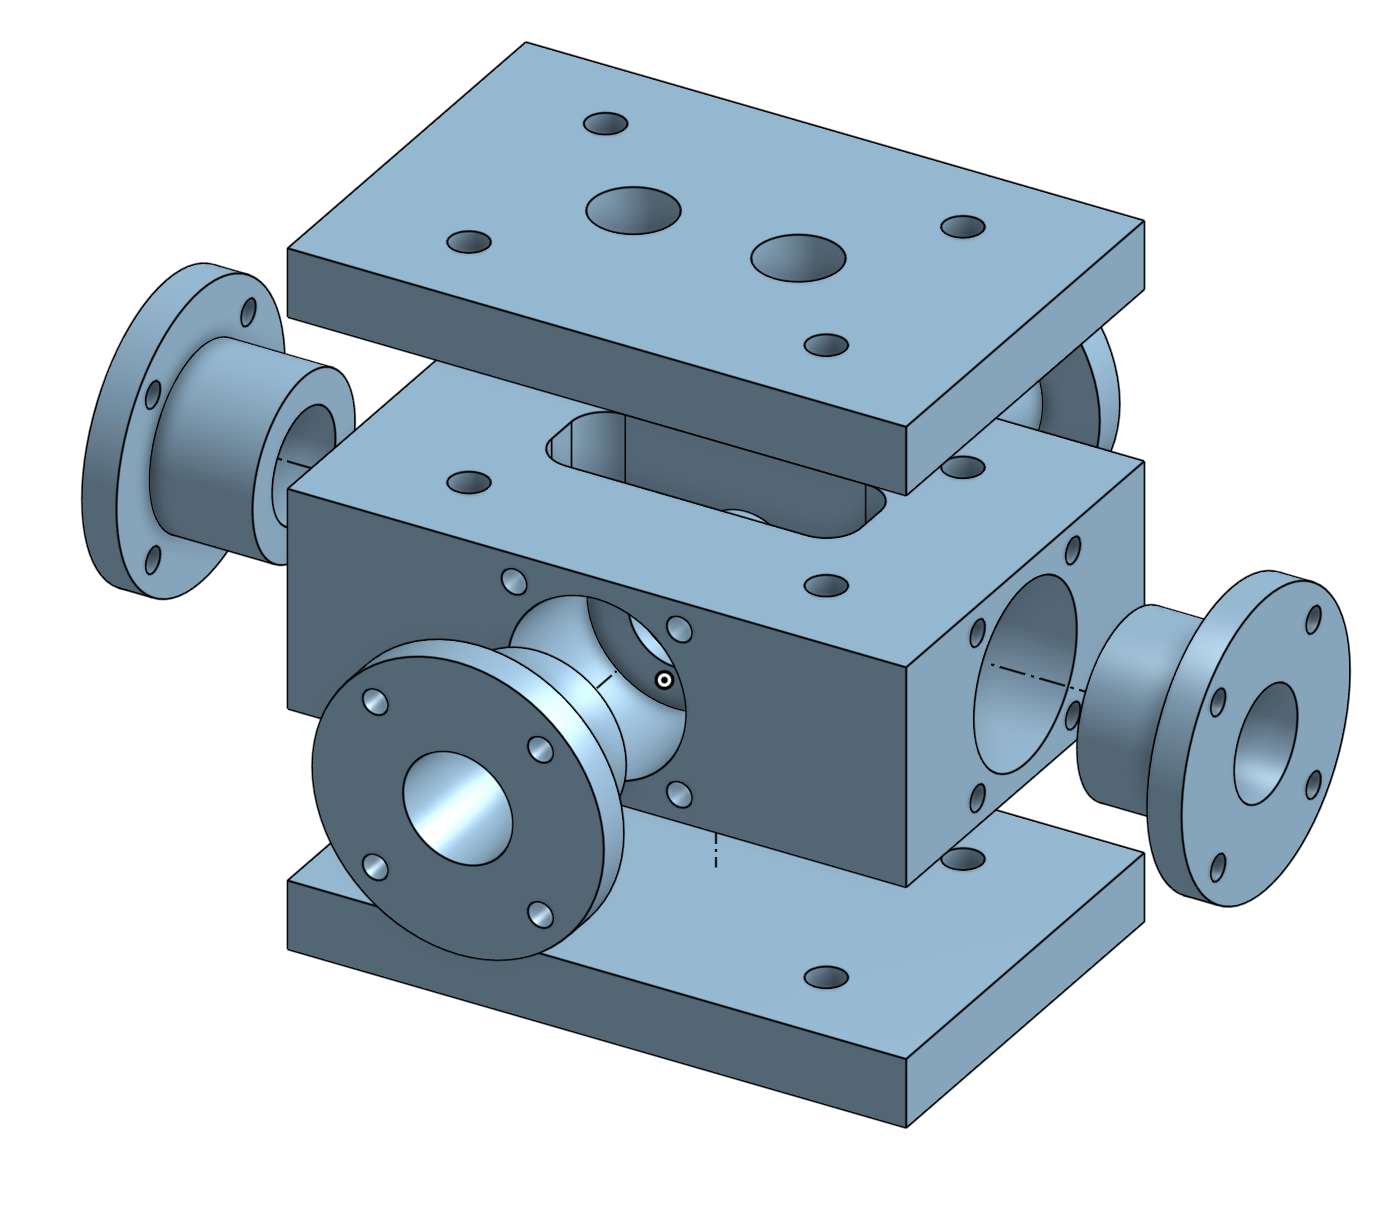
\includegraphics[width=0.8\linewidth]{chapter_4/figures/ftir_box.png}
	\caption{3D CAD model of gas viewing chamber for FTIR.}
	\label{fig:ftir_box}
\end{figure}

%The schematic for the viewing chamber can be seen in figure \ref{}. The main block has four holes along the front, back, left, and right sides for the KBr windows; and chamber along the top to bottom axis for mixing of the gas. The top and bottom blocks were almost identical, with the exception of the top block containing the inlet and outlet holes for the gas. The KBr windows were sealed using rubber o-rings and the machined aluminium holder. Whilst the top and bottom blocks were sealed to the main block using rubber gaskets. This ensured that the chamber was as air-tight as possible.

The dimensions of the viewing chamber will governed the fraction of transmitted light detected by the FTIR. This is due to the optical path length ($l$) of the incident through the sample gas. This relationship is governed by the Beer–Lambert law, seen below:

\begin{equation}
    T = \frac{I}{I_0} = exp(-\mu l)
    \label{eq:beer_lambert_law}
\end{equation}

where $T$ is the transmittance, $I$ is the intensity of light measured, $I_0$ is the light intensity of the incidence light, and $\mu$ is the attenuation coefficient  of the sample. The attenuation coefficient for a given volume is simply the sum of the absorption coefficient ($\mu_a$) and scattering coefficients($\mu_s$). However, since the FTIR is only measuring the amount of light absorbed by the sample, the scattering coefficient can be ignored. The absorption coefficient can also be expressed in terms of the absorption cross section, shown in equation \ref{eq:absorption_cross_section}.

\begin{equation}
    \mu = \sigma n
    \label{eq:absorption_cross_section}
\end{equation}

where $n$ is the number density of the sample, i.e. the number of constituent particles per unit volume. The absorption cross section($\sigma$) is best described as the probability that particles within the sample will absorb the light.

Therefore, equation \ref{eq:beer_lambert_law} can be updated as follows:
\begin{equation}
    T = \frac{I}{I_0} = exp(-\sigma nl)
    \label{eq:beer_lambert_law_with_cross_section}
\end{equation}

The viewing chamber was designed to have two two optical path lengths. One along the length with $l = 5$ cm, and another along the width where $l = 2$ cm. These path lengths were designed to be small to allow greater sensitivity when measuring drop in light intensity.

Typically when using an FTIR, one would first calibrate the device by measuring the background signal. After that, a measurement of the sample can be taken. The FTIR software would then remove the effects of the background signal and return the change in light intensity with sample, called the transmittance (T). The goal would be to continuously take these measurements to detect the change of CO$_2$ concentration in the sample gas. Luckily, the Jasco software has the ability to take continuous measurements over a set interval. 

\begin{figure}[h!]
	\centering
	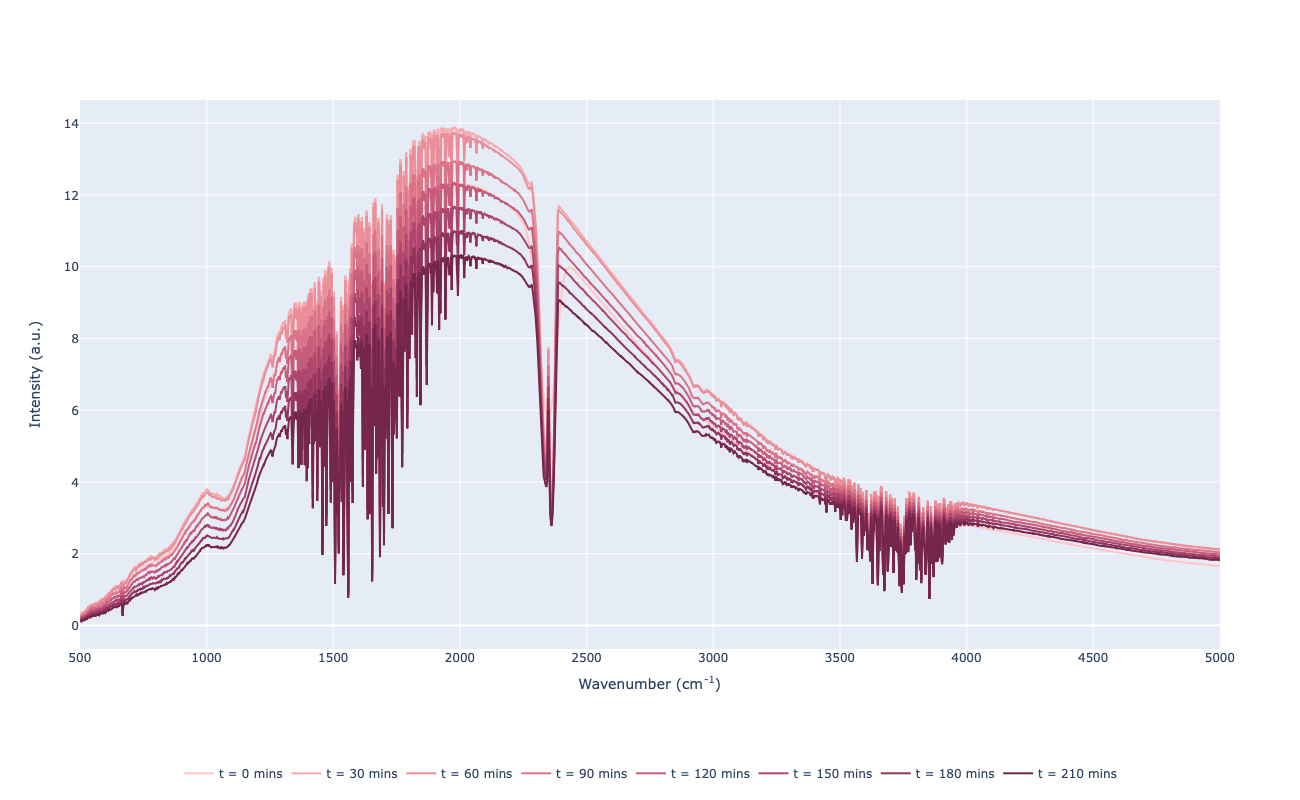
\includegraphics[width=\linewidth]{chapter_4/figures/raw_light_data_shift.png}
	\caption{Snapshots of raw light data from FTIR across the span of 3.5 hours.}
	\label{fig:raw_light_data_shift}
\end{figure}

However when the FTIR is set in this mode, it cannot take another background signal. This is an issue because the concentration of background gas changes over time, which would impact the sample measurement. Another issue present with the device being used is that the characteristics of the incident light intensity changes with time. An illustration of this can be seen in figure \ref{fig:raw_light_data_shift}, showing snapshots of the raw light data from the FTIR after running continuously for 3.5 hours. Another visualisation of this change can be seen in figure \ref{fig:second_moment_of_area}, highlighting the shift of the second moment of area (which can be thought as the centre of mass) of each snapshot over time. Since a 3D plot would be difficult to show in a  report form, the change of wavenumber and intensity are shown in separate axis. The cause of this is uncertain, but it most likely stems from the fact that the optics were not designed to operate in such a continuous fashion.

\begin{figure}[h!]
	\centering
	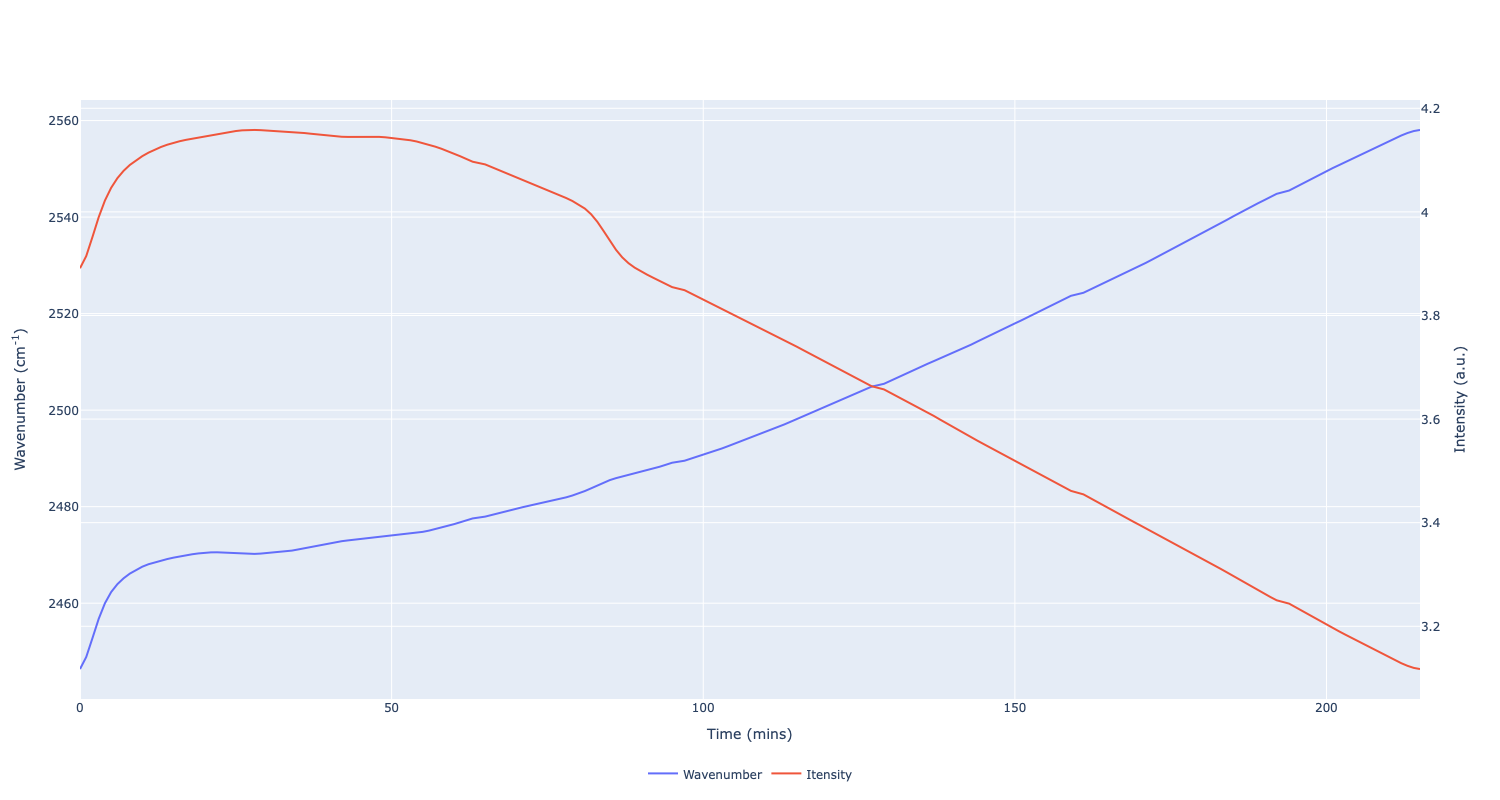
\includegraphics[width=1\linewidth]{chapter_4/figures/second_moment_of_area.png}
	\caption{The change of the second moment of area over the span of 3.5 hours.}
	\label{fig:second_moment_of_area}
\end{figure}

In order to combat both these issues, the computations that would typically be handled by the FTIR software had to be done manually. The first step would be to preprocess the raw light data from the FTIR, shown in figure \ref{fig:raw_light_data_shift}. The data, which can be called $f(\tilde{\nu})$, corresponds to an average signal detected by the FTIR detector for a ``single beam" of light. The jagged peaks located between 1300-2000 cm$^{-1}$ and 3000-4000 cm$^{-1}$ correspond to absorption due to water vapour in the atmosphere, whilst as previously mentioned CO$_2$ absorption can be seen between 2300-2400 cm$^{-1}$. The general structure of these peaks can be captured by filtering the signal. After testing a few different filtering functions, it was found that the Gaussian filter produced the cleanest results. The Gaussian function is expressed as follows:

\begin{equation}
    g(\tilde{\nu}) = \frac{1}{\omega \sqrt{2\pi}} exp \left ( -\frac{\tilde{\nu}}{2 \omega^2} \right )
\end{equation}

where $\omega$ is a specified term that determines the width (or mathematically speaking, the standard deviation) of the impulse. Typically this term is denoted with the symbol $\sigma$, however this has been replaced to avoid any confusion with the absorption cross section seen in equation \ref{eq:absorption_cross_section}. 

\begin{figure}[h!]
	\centering
	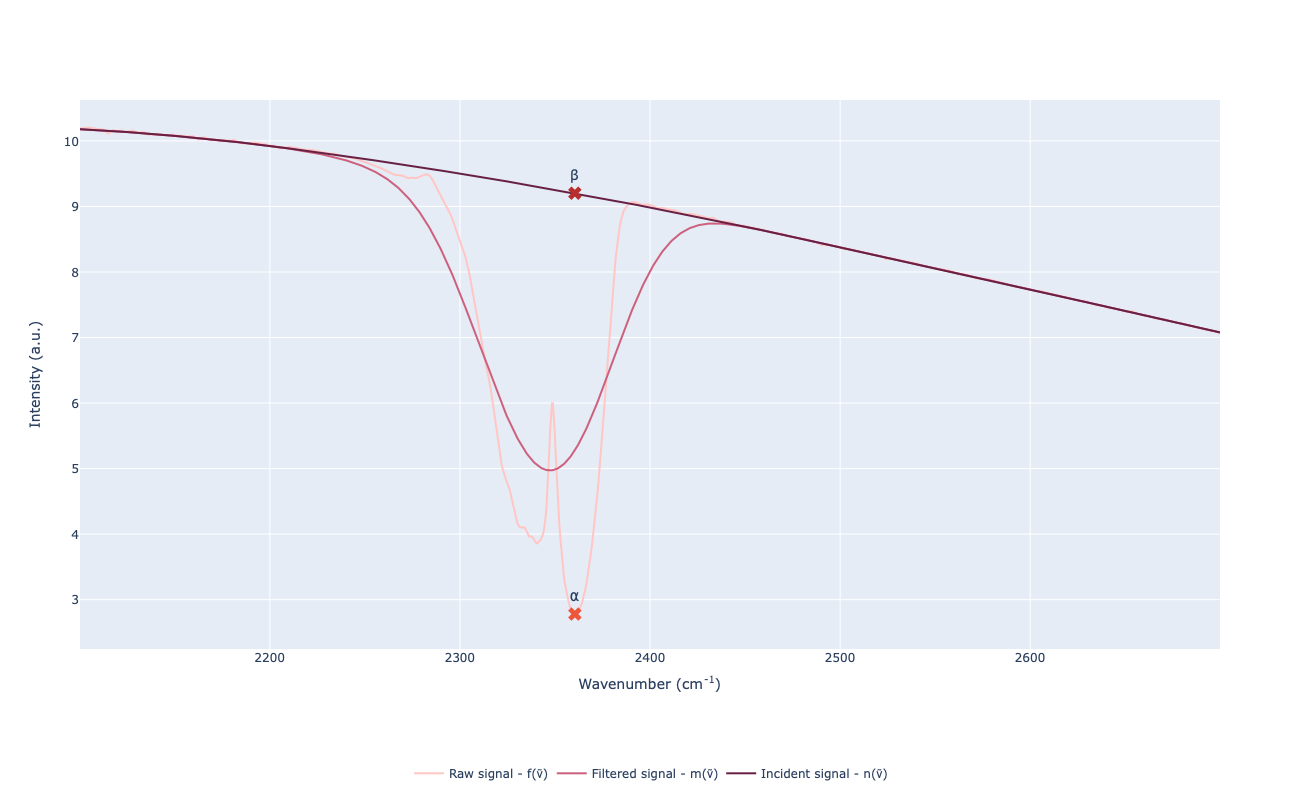
\includegraphics[width=1\linewidth]{chapter_4/figures/FTIR_preprocessing.png}
	\caption{Output signals from FTIR preprocessing steps.}
	\label{fig:FTIR_preprocessing}
\end{figure}

Taking the convolution of the raw signal with the filter, $f(\tilde{\nu}) * g(\tilde{\nu})$, produces a cleaned signal that denotes the general characteristics of the absorption spectra. With this cleaned signal, called $m(\tilde{\nu})$, the focus can be placed to the region that corresponds to the of CO$_2$ absorption. For this, $m(\tilde{\nu})$ can be truncated between 2100-2600 cm$^{-1}$. A comparison between $f(\tilde{\nu})$ and $m(\tilde{\nu})$ in this truncated region can be seen in figure \ref{fig:FTIR_preprocessing}. The final step in the preprocessing was to remove the effects of the CO$_2$ absorption to determine the estimated true incident light signal. This was achieved by first removing the peak from $m(\tilde{\nu})$, then performing a quadratic interpolation of the remaining data points. The interpolation technique used is called spline interpolation and is beyond the scope of this report, however the documentation of the function used can be found in \cite{PresTeukVettFlan92, BSpline_scipy}. The estimated incident signal can be referred to as $n(\tilde{\nu})$.

 With this preprocessing complete, the transmittance of the light from the FTIR can be determined. First, the intensity at the CO$_2$ absorption peak needs to taken from $f(\tilde{\nu})$. For the purposes of this report, the peak of CO$_2$ absorption is said to be at 2360 cm$^{-1}$, and is represented as $I_m$. Next, the incident light intensity is taken from $n(\tilde{\nu})$; also at 2360 cm$^{-1}$. These are denoted in figure \ref{fig:FTIR_preprocessing} as the points $\alpha$ and $\beta$ respectively. With that, the measured transmittance can be determined using:

\begin{equation}
    T_m = \frac{I_m}{I_0} = \frac{\alpha}{\beta}
    \label{eq:measured_transmittance}
\end{equation}

Nevertheless, this only solves one part of the problem. The issue of subtracting out the effects of the background CO$_2$ remains. To solve this, several steps were undertaken during the data gathering stage. First, the region of the FTIR containing the sample and detectors were continuously filled with nitrogen (N$_2$) gas. This would keep the FTIR in positive pressure, minimising the mixing of gas from the atmosphere. However, it would not eliminate the presence of background CO$_2$ present. Then, when gathering the data on different concentration of CO$_2$ in the gas sample, the chamber would be flushed with Helium before the next concentration of CO$_2$ being tested. 

\begin{figure}[h!]
	\centering
	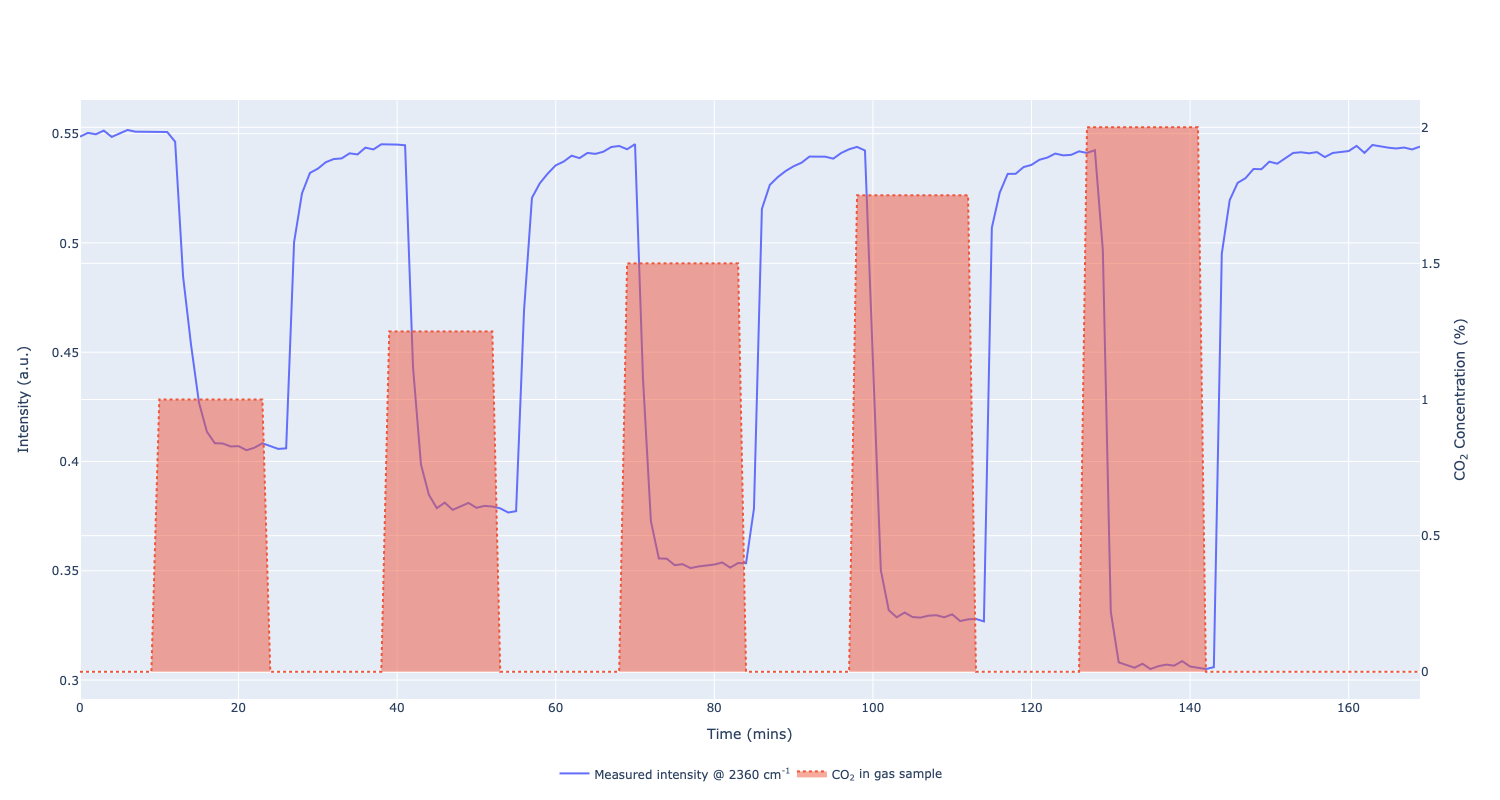
\includegraphics[width=1\linewidth]{chapter_4/figures/time_series_plot_of_transmittance.png}
	\caption{Test measured transmittance at 2360 cm$^{-1}$ across CO$_2$ concentrations between 1-2\%.}
	\label{fig:time_series_plot_of_transmittance}
\end{figure}

A visualisation of this testing process can be seen in figure \ref{fig:time_series_plot_of_transmittance}. It figures shows the transmittance at 2360 cm$^{-1}$ when evaluating CO$_2$ concentrations between 1-2\%, with increments of 0.25\%. Readings from the FTIR were taken approximately every minute, with each test of different CO$_2$ concentrations in the sample lasting 20 mins. This was down to allow sufficient time for the readings to stabilise. While the transient from background took 5-6 minutes in all tests performed, the settling time depends on the flow rate of the mass flow controllers and the volume of the overall experimental setup. 

The reason for flushing the gas in the chamber after every test was to obtain multiple samples of the background transmittance, which can be averaged to determine the reading of the background CO$_2$. The measured transmittance is actually a combination of the CO$_2$ in the gas chamber and the background, which can be expressed as:

\begin{equation}
    T_m = T_b \times T_c = exp(-\sigma n_b l_b) \times exp(-\sigma n_c l_c)
        \label{eq:total_transmittance}
\end{equation}

where the terms with the subscript $b$ correspond to the signal of the background, while terms with the subscript $b$ corresponds to the signal from the CO$_2$ gas sample. $T_m$ is expressed in equation \ref{eq:measured_transmittance}.

By flushing the chamber with Helium, the $n_c$ term goes to zero resulting in the expression for the background transmittance of:

\begin{equation}
    T_b = \frac{I_b}{I_0} = exp(-\sigma n_b l_b)
\end{equation}

This can be substituted into the equation \ref{eq:total_transmittance} giving the an expression for the transmittance due to the sample:

\begin{equation}
    T_c = \frac{I_c}{I_b} = exp(-\sigma n_c l_c)
    \label{eq:sample_transmittance}
\end{equation}

The test procedure shown in figure \ref{fig:time_series_plot_of_transmittance} was repeated across many different CO$_2$ concentrations between a 0.25 to 5\% CO$_2$-Helium mixture, with a greater test frequency placed on values between 0.25 to 2\% since this is the region of operation for the SRR. The results of these test are shown in figure \ref{fig:co2_conc_absorbance}, which shows the relationship between the CO$_2$ concentration and the absorbance. The absorbance is a simplification of the terms within the exponential, $A = -\sigma n l$; and can also be defined as $ln (T_c)$. The absorbance is also directly proportional to the CO$_2$ concentration, as changing the flow rate of gas changes the number density of CO$_2$ molecules in the gas sample. This relationship is also shown in figure \ref{fig:co2_conc_absorbance}, where a line of best fit was plotted using the least-square solution. The rational for using this instead of a traditional regression fit was to force the solution through the origin.


\begin{figure}[h!]
	\centering
	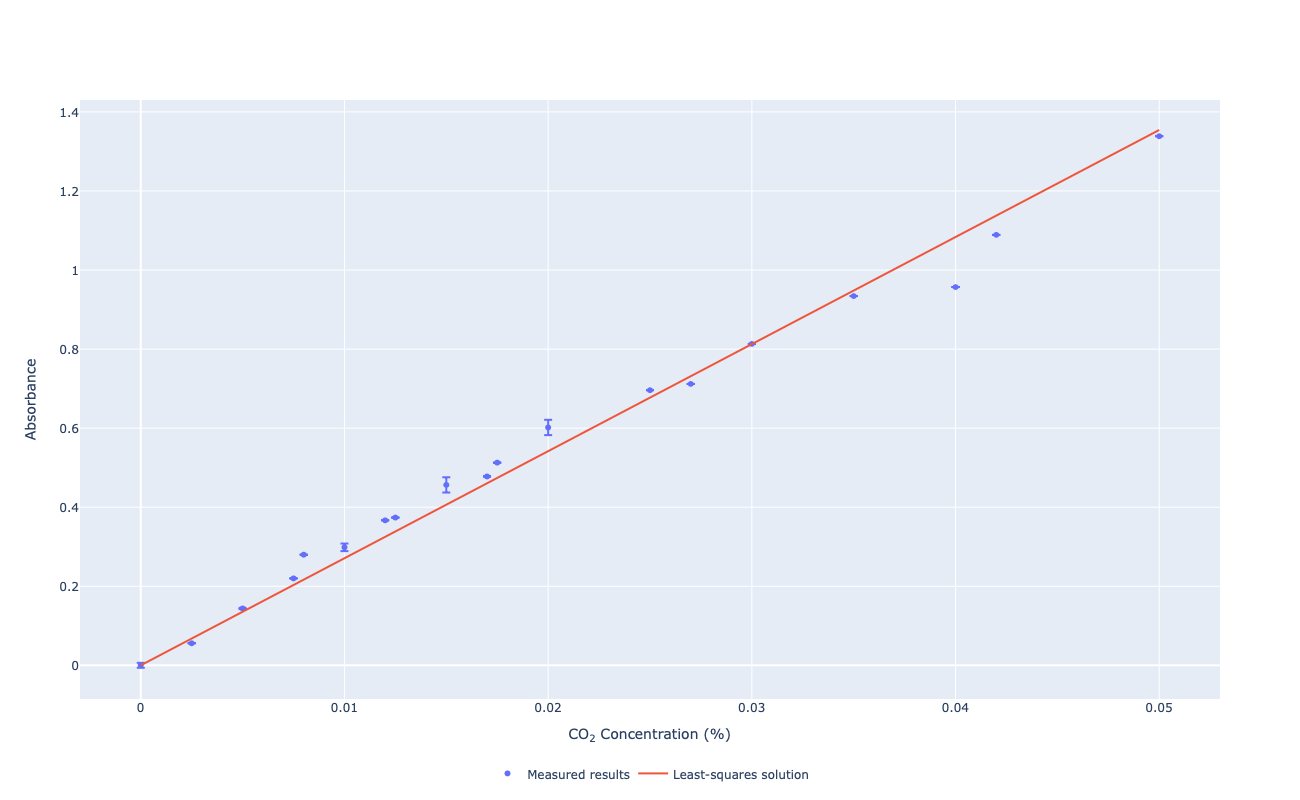
\includegraphics[width=1\linewidth]{chapter_4/figures/co2_conc_absorbance.png}
	\caption{Absorbance across CO$_2$ concentrations between 0-5\%.}
	\label{fig:co2_conc_absorbance}
\end{figure}







